\documentclass[11pt,a4paper,titlepage]{article}
\usepackage[utf8]{inputenc}
\usepackage{amsmath}
\usepackage{amsfonts}
\usepackage{adjustbox}
\usepackage{csvsimple}
\usepackage{amssymb}
\usepackage{hyperref}
\hypersetup{
    colorlinks=true,
    linkcolor=black,
    filecolor=black,
    urlcolor=cyan,
    citecolor=black,
}

\usepackage{tikz}
\usetikzlibrary{calc,patterns,angles,quotes,shapes.geometric, arrows}
\tikzstyle{train} = [rectangle, rounded corners, minimum width=2.2cm, minimum height=1cm,text centered, draw=black, fill=red!30]
\tikzstyle{test} = [rectangle, rounded corners, minimum width=2.2cm, minimum height=1cm,text centered, draw=black, fill=green!30]
\tikzstyle{data} = [rectangle, rounded corners, minimum width=11.8cm, minimum height=1cm,text centered, draw=black, fill=gray!30]
\tikzstyle{MSE} = [rectangle, rounded corners, minimum width=1.4cm, minimum height=1cm,text centered, draw=black, fill=orange!30]
\tikzstyle{arrow} = [thick,->,>=stealth]

\usepackage{float}
%\usepackage{mathtools}
\usepackage{bm}
\usepackage[margin=1in]{geometry}

\title{Project 1 in FYS-STK4155}
\author{Adrian Martinsen Kleven & Simon Elias Schrader }
\date{Autumn 2020}
\usepackage{hyperref}

\usepackage{natbib}
\usepackage{graphicx}
\graphicspath{{../figures/presentable_data/}} %Setting the graphicspath

\begin{document}
\maketitle
\tableofcontents
\listoffigures
\listoftables

\clearpage
\section{Abstract}
In almost all fields of science, extrapolating data and creating a fitting function in a reliable way, is tremendously important, and thanks to computers, doing so is increasingly possible using automatized methods. Using existing OLS, Ridge, and LASSO regression, we fitted the Franke Function \eqref{FrankeFunction} with added noise and geographic data with 2D polynomials of varying degrees and analysed different statistical values of interest. We found that OLS is prone to overfitting due to a very large variance at high complexities, while Rigde and LASSO remain stable at these higher degrees. With our parameters \& data, Ridge and OLS regression gave about the same Mean Square Error (MSE), while LASSO did not converge to a desirable value at higher polynomial degrees and hence gave larger errors. For the geographical data, we found that, with 50,000 randomly chosen data points, using  OLS regression, the MSE is around 18,000 at the ideal value, while using Ridge regression, it is ~16,500. Hence, regression does not seem to be suitable for predicting geographical data, but manages to include the general traits. We also compared k-fold Cross Validation to Bootstrap and found out that these two methods do not give the same error estimates. 
%In this project, we use some good methods and some shitty methods to test how well a polynomial can interpolate a superfancy exponential function (protip: It can't) . Then we use the same approaches to see how well random geographic data can be approximated. We expect this to look horrible. We're sorry for abusing math in that way. We shall contemplate Seppuku.

%\begin{figure}[H]
%\centering
%
\includegraphics[scale=1.7]{universe}
%\caption{Some random picture.}
%\label{fig:universe}
%\end{figure}


\section{Introduction}
The purpose of this article is to explore three different linear regression algorithms, their utility, application and some of the theory behind them. These are Ordinary Least Squares (OLS), as well as the two Shrinkage methods Ridge regression and LASSO regression.In this article, we compare these methods to one another and see how well they perform for the given problems, as well as describe their applicability and their peculiarities. These methods are tested on a model dataset constructed using the Franke function \eqref{FrankeFunction} with added normally distributed noise, then later applied to digital terrain data over a part of South Korea in an attempt to accurately recreate the image. We explore the two resampling techniques K- fold cross validation and Bootstrap and compare the error estimates achieved by both methods and compare their runtime. We study the Bias-Variance Tradeoff and prove that the Mean Square Error can be decomposed into an irreducible part, the squared Bias, and the Variance. Resampling is usually used for models where the amount of data is restricted. Seeing as terrain data has a finite resolution, its application should be considered for error estimation or model selection although we don't cover this. The models we consider are not limited by lack of data, but resampling is nevertheless a valid method for predicting various statistical values.\\\\All methods are implemented using the Python programming language. The programs are available at the \href{https://github.com/schraderSimon/FYS-STK/tree/master/project1}{Github address}.
\section{Methods}

\subsection{Linear Regression}
The aim of Linear Regression is to find the conditional distribution $p(y|\bm{x})$ for y given $\bm{x}$. In Linear Regression, a linear functional dependence is assumed, and the aim is hence to create a linear function that fits a set of $p$ predictor variables $\bm{x}$ to a target variable $\bm{y}$, where there are $n$ discrete observations for each of the $p$ predictor variables and the target variable. That is, the aim is to find a functional relationship of the form $f(\bm{x})=y$. \\
We assume hence that each target variable $y_i$ has a functional dependence of the predictor variables:
\begin{equation*}
y_i= \tilde{y}_i+\epsilon_i=\beta_0 + \beta_1x_{i0} + \beta_2x_{i1}+...+\beta_px_{i(p-1)} + \epsilon_i
\end{equation*}
As this is true for all y, this can be written in matrix form:
\begin{equation*}
\bm{y}= \bm{X\beta} + \bm{\epsilon}
\end{equation*}
where $\bm{y}$, and $\bm{\epsilon}$ are vectors of length n,  $\bm{\beta}$ is of length p and $\bm{X}$ is a matrix of size $n*p$. X is called the design matrix.
 We now want to find fitting parameters $\bm{\beta}$ that represent the best linear fit of y to the input data $\bm{x}$. Hence, we want the fit
 \begin{equation*}
 \bm{\tilde y}= \bm{X\beta}
 \end{equation*}
 to be as close to the target data $\bm{y}$ as possible.
  There are several approaches to define the best linear fit, and in this article, we looked at three different methods that define the best fit in a different way each. All methods have in common that they define a loss function, which describes the deviation from the fit to the real data, that needs to be minimized.
\subsubsection{Statistical quantities}
Before explaining these three methods, it is of importance to define statistical quantities to evaluate the quality of a fit.
The Mean Square Error (MSE) is defined as 
\begin{equation}\label{MSE}
MSE(\bm{y},\bm{\tilde y})=\frac{1}{n}\sum_i^N\left(y_i - \tilde y_i \right)^2=\mathbb{E}\left[(\bm{y}-\bm{\tilde y})^2  \right]
\end{equation}
where the left formula is the within-sample mean square error and $\bm{\tilde y}$ and $\bm{y}$ are vectors. It describes hence the average/expected square of the deviation between to vectors. It is equal to zero if and only if two vectors are identical.\\
The $R^2$-score is defined as 
\begin{equation}\label{R2}
R^2(\bm{y}, \bm{\tilde y}) = 1 - \frac{\sum_{i=0}^{n - 1} (y_i - \tilde{y}_i)^2}{\sum_{i=0}^{n - 1} (y_i - \bar{y})^2},
\end{equation}
where we have defined the mean value  of $\bm{y}$ as
\[
\bar{y} =  \frac{1}{n} \sum_{i=0}^{n - 1} y_i
\]
The $R^2$-score is equal to 1 if and only if the two arrays are identical, and values close to 1 indicate that two vectors are similar (or that a fit is good). 
The Variance $\sigma^2$ is defined as 
\begin{equation}\label{variance}
\sigma^2=\mathbb{E}\left[(X-\mathbb{E}\left[X\right])^2\right]
\end{equation}
for a random variable X. When fitting the Franke Function \ref{FrankeFunction}, $\sigma^2$ is known, however, when fitting the terrain data, it has to be estimated. The following estimator is used:
\begin{equation}\label{variance_estimate}
\hat\sigma^2 = \frac{1}{N-p-1}\sum\limits_{i=1}^N(y_i-\bar{y}_i)^2
\end{equation}

where $N-p-1$ is the degrees of freedom. and p is the number of input variables in the regression model.
\subsubsection{Ordinary Least Squares (OLS) Regression}
In Ordinary Least Square regression, the loss function is defined as the following:
\begin{equation*}
C(\bm{\beta})= \frac{1}{n}\sum_{i=0}^n\left( y_i-\tilde y_i \right)^2
=\frac{1}{n}(\bm{y}-\bm{\tilde y})(\bm{y}-\bm{\tilde y})^T=
\frac{1}{n}(\bm{y}-\bm{X\beta})(\bm{y}-\bm{X\beta})^T
\end{equation*}
The solution minimizing this problem is found by deriving $C(\bm{\beta})$ with regards to each $\beta_i$ and setting each derivative equal to zero. Doing this, we end up with the following equation (in matrix notation)
\begin{equation*}
\frac{\partial C(\bm{\beta})}{\partial\bm{\beta}}=0=\bm{X^T}(\bm{y}-\bm{X\beta})
\end{equation*}
which gives us
\begin{equation*}
\bm{\beta}=(\bm{X}^T\bm{X})^{-1}\bm{X}^T\bm{y}
\end{equation*}
which can be solved when $(\bm{X}^T\bm{X})$ is invertible. In the case of strongly correlated data and large matrices, There might be issues in inverting $(\bm{X}^T\bm{X})$ due to the matrix being singular. Also, for very large matrices, there might be issues caused by the fact that many mathematical operations can introduce a numerical error. Hence, an equivalent, but more stable way to implement the solution for $\bm{\beta}$ is to use Singular Value Decomposition (SVD). As every matrix has a SVD decomposition, we can write
\begin{equation}\label{SVD_OLS}
\begin{split}\bm{\beta} & =\left(\bm{X}^T\bm{X}\right)^{-1}\bm{X}^T\bm{y}\\
& = \left(\bm{V}\bm{D}^T\bm{U}^T\bm{U}\bm{D}\bm{V}^T\right)^{-1}\bm{V}\bm{D}^T\bm{U}^T\bm{y}\\
& = \left(\bm{V}\bm{D}^T\bm{I}_p\bm{D}\bm{V}^T\right)^{-1}\bm{V}\bm{D}^T\bm{U}^T\bm{y}\\
& = \left(\bm{V}\bm{D}^2\bm{V}^T\right)^{-1}\bm{V}\bm{D}^T\bm{U}^T\bm{y}\\
& = \bm{V}\bm{D}^{-2}\bm{V}^T\bm{V}\bm{D}^T\bm{U}^T\bm{y}\\
& = \bm{V}\bm{D}^{-1}\bm{U}^T\bm{y}\end{split}
\end{equation}.

Under the assumption that true data y is given as
\begin{equation*}
\bm{y}=f(\bm{x})+\bm{\epsilon}
\end{equation*}
where $\bm{\epsilon}$ follows a normal distribution $N(0,\sigma^2)$, information about the variance and the expectation value can be deduced. Assuming that $f(\bm{x})=\bm{X\beta}$, it is easily shown that
\begin{equation*}
\mathbb{E}(y_i)=\bm{X_{i,*}\beta}
\end{equation*}

\begin{equation*}
Var(y_i)=\sigma^2
\end{equation*}

where $\bm{X_{i,*}}$ is the i-th row of the design matrix.

For $\beta$, it can be shown that \citep{HW2}
\begin{equation*}
\mathbb{E}(\bm{\beta})=\bm{\beta}
\end{equation*}
\begin{equation*}
Var(\bm{\beta})=\sigma^2(\bm{X}^T\bm{X})^{-1}
\end{equation*}
\subsubsection{Ridge regression}
The above mentioned problems with OLS regression, namely those of correlated data and near singular matrices, can be amended by implementing ridge regression. This is done by introducing the regularization parameter $ \lambda$ in the cost function:
\begin{equation*}
    C(\boldsymbol{X},\boldsymbol{\beta})=\frac{1}{n}\left\{(\boldsymbol{y}-\boldsymbol{X}\boldsymbol{\beta})^T(\boldsymbol{y}-\boldsymbol{X}\boldsymbol{\beta})\right\}+\lambda\boldsymbol{\beta}^T\boldsymbol{\beta}
\end{equation*}
effectively imposing a penalty on the size of $\boldsymbol{\beta}$. One of the consequences of Ridge regression is that it "shrinks" the singular values $\sigma$ of the Design matrix X: It can be shown that \citep{hastie01statisticallearning}
\begin{equation*}
\bm{y}^{OLS}=\bm{X\hat\beta}^{OLS}=\bm{UU}^T\bm{y}
\end{equation*}
\begin{equation*}
\bm{y}^{Ridge}=\bm{X\hat\beta}^{Ridge}=\sum_{j=1}^{p}\bm{u}_j\frac{\sigma_j^2}{\sigma_j^2+\lambda}\bm{u}^T_j\bm{y}
\end{equation*}
where $\bm{u}_j$ are the column of the matrix $\bm{U}$ from the SVD of $\bm{X}$. It also follows directly from this formula that the smaller singular values are shrunk more.\\
This has the side effect of decreasing the variance of the parameters $\beta$, as well as the values $\beta$ themselves (it can be shown \citep{Ridge_Lecture_Notes} that the variance for all $\lambda>0$ is always lower than when using OLS), and thereby reducing the impact of overfitting.\\We later show the dependence that the variance of $\beta$ has on the regularization parameter. To do this, we need an expression to estimate the variance of our predictions for the $\beta$'s. It's given by $\sigma^2(\hat{\beta}_j) = \sigma^2[X^TX+\lambda \hat{I}]^{-1}_{jj}$\cite{HW1}\cite{HW2}, meaning the diagonal elements of the matrix computed as part of Ridge with matrix inversion. Here, $\sigma^2$ could be estimated by equation \eqref{variance_estimate}\citep{hastie01statisticallearning}, however in our case, the value of $\sigma^2$ is known, as we're the ones constructing the data set.\\The expression for the optimal value of $\boldsymbol{\beta}$ becomes

\begin{equation*}
    \boldsymbol{\beta}^{\mathrm{Ridge}} = \left(\boldsymbol{X}^T\boldsymbol{X}+\lambda\boldsymbol{I}\right)^{-1}\boldsymbol{X}^T\boldsymbol{y}.
\end{equation*}
Where as before the matrix $\boldsymbol{X}^T\boldsymbol{X}$ could have been singular, by adding a non- zero, positive value to the diagonal, the eigenvalues become positive definite ensuring that the matrix is invertible.
\paragraph*{Regularization parameter}
There are several factors that determine how different regularization parameters $\lambda$ will minimize the cost function. A dataset with a lot of noise will cause more overfitting at higher model complexities. We expect that increasing the noise parameter $\sigma$ in a model dataset will make models with a larger value of $\lambda$, perform better. We see an example of this in figure \ref{lambdatonoise}, where models with higher values of $\lambda$ give the smallest MSE with increasing noise.
\begin{figure}[H]
\centering

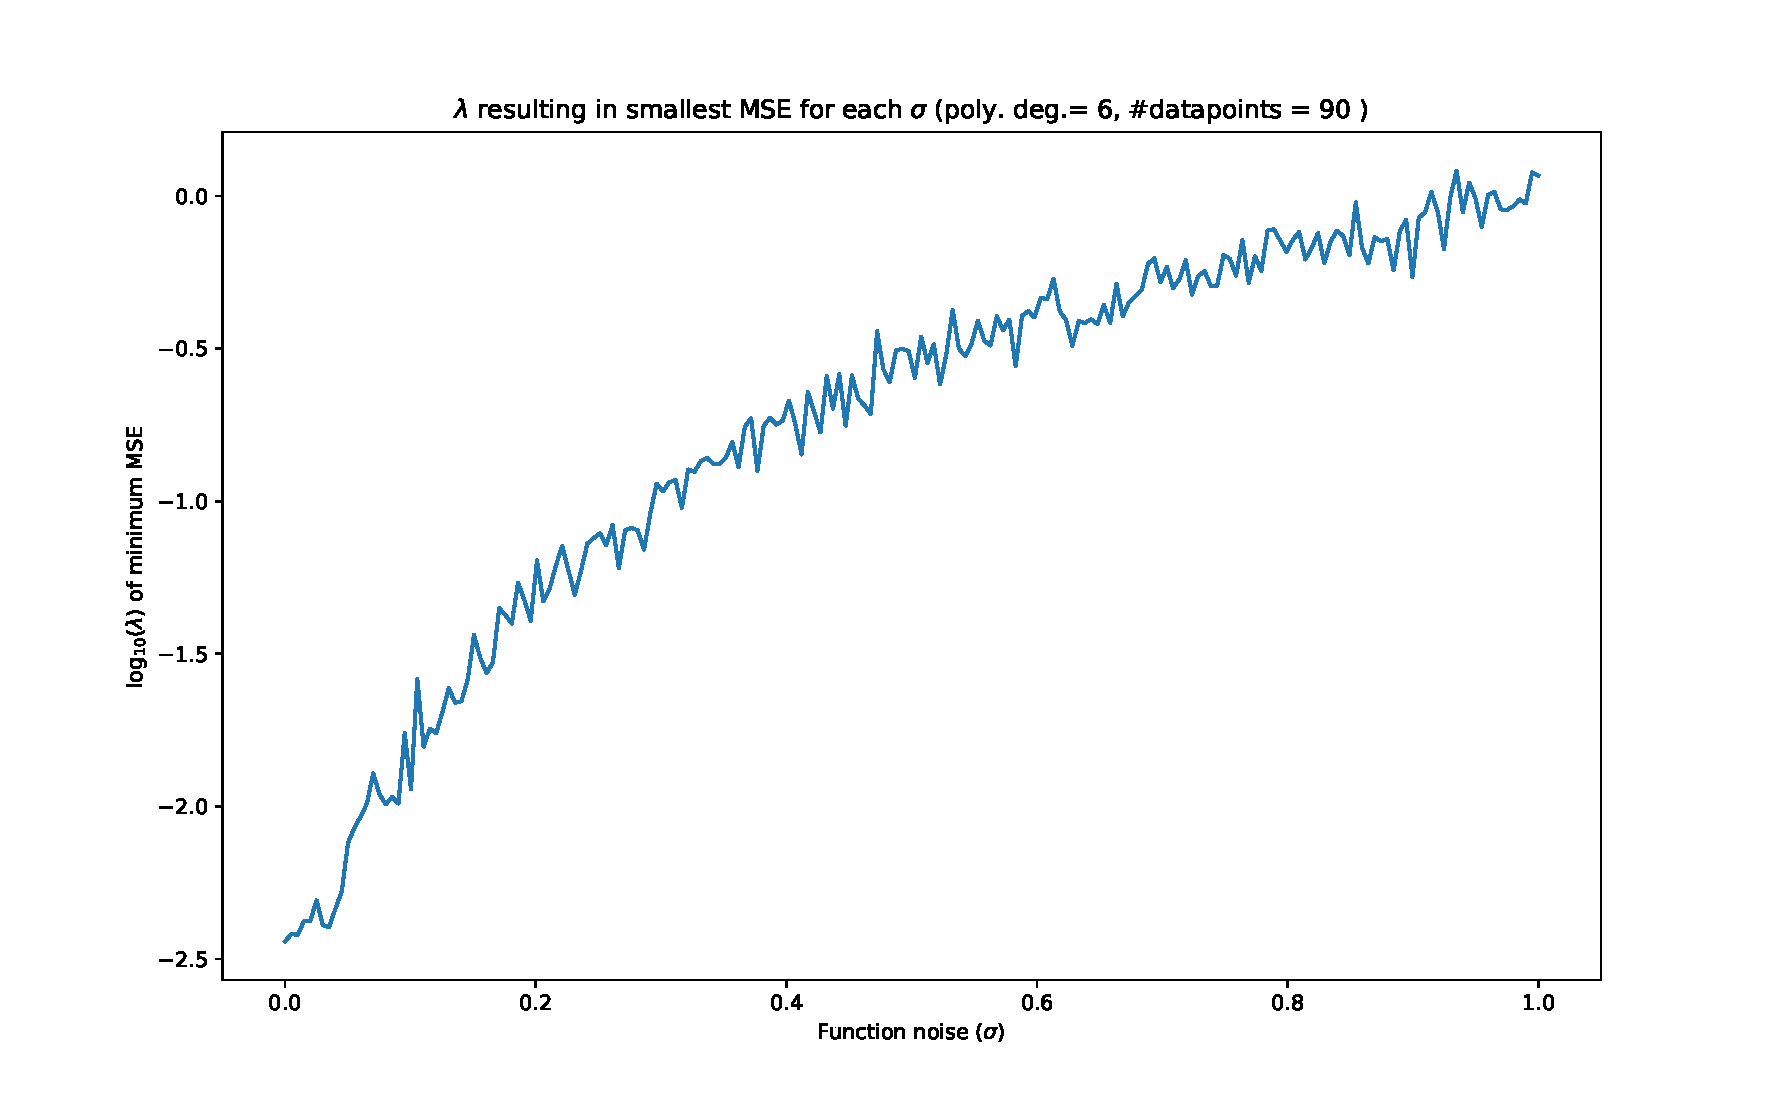
\includegraphics[trim=2cm 1.0cm 2cm 1.4cm, clip=true,scale = 0.5]{Smallest_MSE_lambda_over_noise.pdf}
\caption[Optimal regularization parameter to noise]{Performing Ridge regression on the Franke function \eqref{FrankeFunction}, with a normally distributed error term $\epsilon$.}\label{lambdatonoise}
\end{figure}
\subsubsection{LASSO regression}
As with ridge, LASSO regression implements a new component to the cost function. Only, in this case the penalty is proportional to the L1- norm $\vert\vert \boldsymbol{\beta}\vert\vert$:
\begin{equation*}
    C(\boldsymbol{X},\boldsymbol{\beta})=\frac{1}{n}\left\{(\boldsymbol{y}-\boldsymbol{X}\boldsymbol{\beta})^T(\boldsymbol{y}-\boldsymbol{X}\boldsymbol{\beta})\right\}+\lambda\vert\vert \boldsymbol{\beta}\vert\vert.
\end{equation*}
One of the problems with ridge regression is that rather than eliminating covariant features, it will tend to shrink parameters, reducing their influence but not removing them. This is due to the behaviour of the squaring term in the L2- norm, which penalizes few large numbers more than many small numbers. For example, $\vert\vert[\beta_1,\beta_2]\vert\vert_2 \leq \vert\vert[\beta_1+\beta_2,0]\vert\vert_2$. Whereas in LASSO, the area of the L1- norm in the parameter space is more likely to intersect the least square loss function along the orthogonal axes in the paramater space, along which, at least one of the parameters are zero. This has a greater effect on eliminating features in a model, although which of two collinear parameters are eliminated is arbitrary.
\subsection{Resampling Methods and Data Splitting}
In order to get an approximate estimate of the quality of a fit, it is necessary that the fit is tested on a set that it has not been trained on. As the training set determines the parameters $\bm{\beta}$, we need a set from the same distribution as the training set, which is different from the training set. For that reason, the full data set of predictors and targets is split into a test set and a training set. The test usually contains $20-25\%$ of the full set, while the training set contains $75-80\%$. It is also possible to use a further validation set to do a final estimate using data that has never been "seen" by the programmer or the code, however, this was not implemented in this project.
\subsection{Bias-variance relationship}
In order to evaluate the quality of a fit, it is customary to evaluate the Mean Square Error (MSE) of the test data to the prediction. It is given by \ref{MSE}.
The Mean Square Error can be decomposed into three parts: The unavoidable error $\sigma^2$, the squared Bias (which is the deviation of the mean value of an estrefimator and the true value), and the Variance (which is a measure of the spread of the estimator). Hence
\begin{equation*}
MSE(\bm{y},\bm{\tilde y})=Bias[ \bm{\hat y}]^2 + Var[ \bm{\tilde y}]+\sigma^2= \left(f-\mathbb{E}(\tilde f)\right)^2 + \mathbb{E}\left(\left[\mathbb{E}\left[ \tilde f \right]-f\right)^2 \right]+\sigma^2
\end{equation*}
A proof of this decomposition can be found in the appendix \eqref{Proof}.
In this article, we will however calculate the following values:
\begin{equation*}
Bias[\bm{\tilde y}]^2=\frac{1}{n}\sum_i^N\left( y_i - avg( \bm{\tilde y})\right)^2
\end{equation*}
\begin{equation*}
Var[\bm{\tilde y}]^2=\frac{1}{n}\sum_i^N\left(\tilde y_i - avg( \bm{\tilde y})\right)^2
\end{equation*}
Where $avg()$ stands for the average value.This is because the true values $f_i$ are not known and thus impossible to obtain.\\
An important observation when fitting the data is that the Bias decreases as the model gets more complex, while the variance increases. When the Bias is large, important relations of the underlying data are not considered. When the Variance is high, small, unimportant features in the training set have too high of an impact. This is called overfitting. The aim is hence to find the model complexity that gives the lowest MSE. This is usually the case around the point where the Bias has the same magnitude as the Variance.
\subsubsection{Bootstrap method}
The Bootstrap method is a method that can be used to calculate statistical quantities. The main idea is the following: Let n be the size of the training set $Z=(z_1,z_2,...z_n)$, where each $z_i$ contains p predictors and one target value, that is $z_i=(x_{i,1},x_{i,2},...x_{i,p},y_i)$. Now, n data points $z_i$ are drawn randomly from Z with replacement. This is done $B$ times, creating $B$ new sets $Z'_j$. We can now create a fitting model for each of the sets  $Z'_j$. For each of these data sets $Z'_j$, we can now calculate any variable $\hat\theta_j$ given the data. Now, the distribution of $\hat\theta_j$ can be used to estimate the distribution of $\theta$ and get values of interest, such as the mean value or the variance. In this article, Bootstrap is used to get information about the test MSE, variance and bias in order to evaluate the quality of the fit. This is done by using the B bootstrap sets $Z'_j$ to calculate the fitting parameters $\beta$ and calculate B fits to the test set. $\tilde{Y_j}$. From these B fits, we can then approximate the test MSE, variance and bias.
\subsubsection{K-fold Cross validation}
K- fold Cross Validation is a useful technique for when you have a limited data set, and want to make sure that all features are captured in a training set. K- fold Cross Validation does this by partitioning the data set into $k$ so called folds, assigning $k-1$ folds as the training set and $1$ of the folds as the testing set. It does this $k$ times, making sure to utilize each fold as the testing set once, as seen in figure \ref{kfoldcrossillustrated}. In this way, we end up generating $k$ different models, whose performance can be measured with respect to the testing fold or additionally, a separate testing set withheld from the partitioning process.

\begin{figure}[H]
\centering
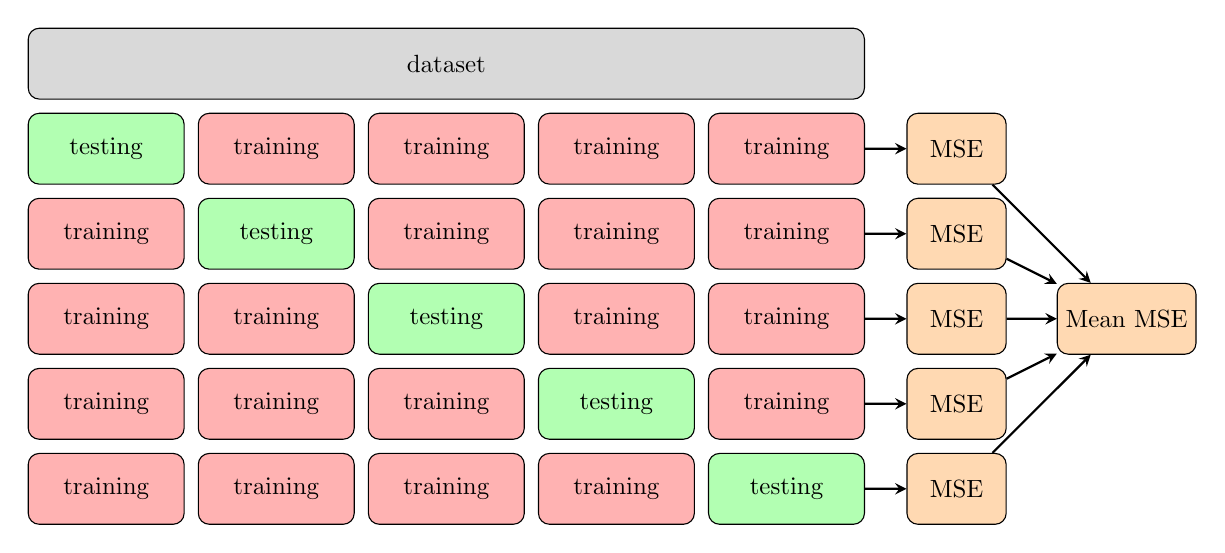
\begin{tikzpicture}[node distance=2.4cm,scale=0.9, every node/.style={scale=0.9}]

\node (data1)[data]{dataset};
\node (test1)[test,below of =data1,yshift =1.2cm,xshift=-4.8cm]{testing};
\node (train1) [train,right of=test1] {training};
\node (train2) [train,right of=train1] {training};
\node (train3) [train,right of=train2] {training};
\node (train4) [train,right of=train3] {training};
\node (MSE1) [MSE,right of=train4] {MSE};
\draw [arrow] (train4) -- (MSE1);

\node (test12)[train,below of =test1,yshift =1.2cm]{training};
\node (train12) [test,right of=test12] {testing};
\node (train22) [train,right of=train12] {training};
\node (train32) [train,right of=train22] {training};
\node (train42) [train,right of=train32] {training};
\node (MSE2) [MSE,right of=train42] {MSE};
\draw [arrow] (train42) -- (MSE2);

\node (test13)[train,below of =test12,yshift =1.2cm]{training};
\node (train13) [train,right of=test13] {training};
\node (train23) [test,right of=train13] {testing};
\node (train33) [train,right of=train23] {training};
\node (train43) [train,right of=train33] {training};
\node (MSE3) [MSE,right of=train43] {MSE};
\draw [arrow] (train43) -- (MSE3);

\node (test14)[train,below of =test13,yshift =1.2cm]{training};
\node (train14) [train,right of=test14] {training};
\node (train24) [train,right of=train14] {training};
\node (train34) [test,right of=train24] {testing};
\node (train44) [train,right of=train34] {training};
\node (MSE4) [MSE,right of=train44] {MSE};
\draw [arrow] (train44) -- (MSE4);

\node (test15)[train,below of =test14,yshift =1.2cm]{training};
\node (train15) [train,right of=test15] {training};
\node (train25) [train,right of=train15] {training};
\node (train35) [train,right of=train25] {training};
\node (train45) [test,right of=train35] {testing};
\node (MSE5) [MSE,right of=train45] {MSE};
\draw [arrow] (train45) -- (MSE5);

\node (MSEtot) [MSE,right of=MSE3] {Mean MSE};
\draw [arrow] (MSE1) -- (MSEtot);
\draw [arrow] (MSE2) -- (MSEtot);
\draw [arrow] (MSE3) -- (MSEtot);
\draw [arrow] (MSE4) -- (MSEtot);
\draw [arrow] (MSE5) -- (MSEtot);


\end{tikzpicture}
\caption[K-fold Cross Validation operation structure]{In this example, 5- fold Cross Validation is used on the entire dataset, with one model being generated for each row. The MSE on the test set is then calculated and averaged with the MSEs of every other model.}\label{kfoldcrossillustrated}
\end{figure}
The value we choose for $k$ will impact the accuracy of our model. To see this, we performed OLS regression on the same function \eqref{FrankeFunction} using different values for $k$ resulting in figure \ref{bestKOLS}.
\begin{figure}[H]
\centering

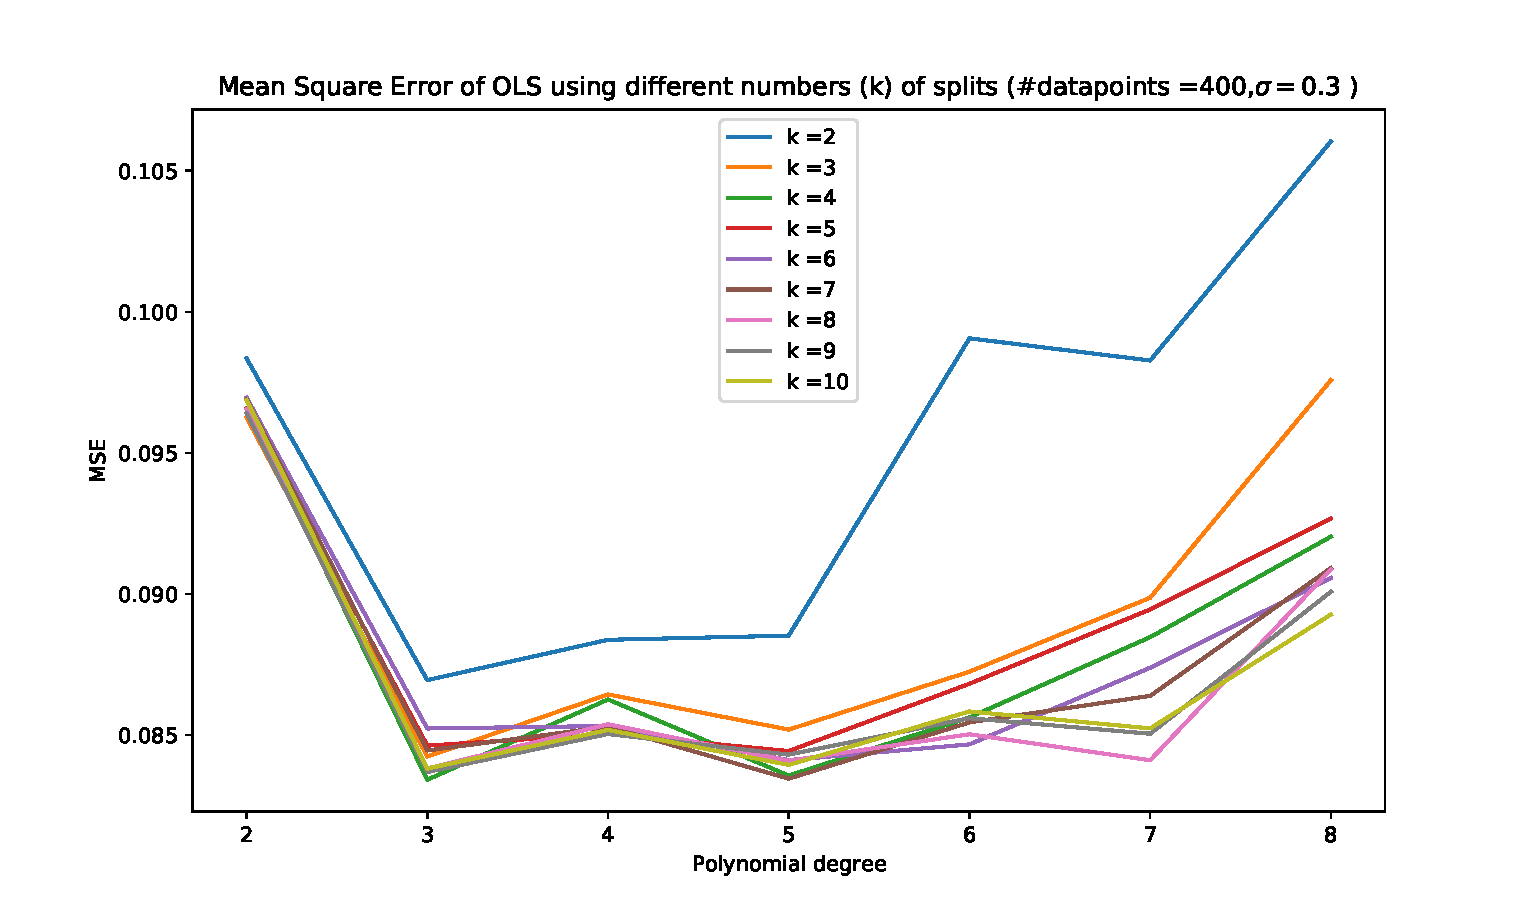
\includegraphics[trim=1.4cm 0.2cm 2.5cm 1.2cm, clip=true,scale = 0.6]{MSE_OLS_k_comparison_2to10.pdf}
\caption[Estimated MSE from OLS using different number of splits in k-fold CV]{Estimated MSE as a function of model complexity (polynomial degree) for different values of $k$, using k- fold CV OLS on the Franke function \eqref{FrankeFunction}. We can see that higher values of $k$ consistently make lower error estimates though there is no clear correlation among the highest few values.}\label{bestKOLS}
\end{figure}
We expect to see this trend based on the increasing size of the training set from $50\%$ to $75\%$ aso. going from $k=2$ to $k=3$ and on.
\subsection{Fitting the Franke function}
The Franke Function is given by
\begin{align}\label{FrankeFunction}
f(x,y) &= \frac{3}{4}\exp{\left(-\frac{(9x-2)^2}{4} - \frac{(9y-2)^2}{4}\right)}+\frac{3}{4}\exp{\left(-\frac{(9x+1)^2}{49}- \frac{(9y+1)}{10}\right)}\nonumber \\
&+\frac{1}{2}\exp{\left(-\frac{(9x-7)^2}{4} - \frac{(9y-3)^2}{4}\right)} -\frac{1}{5}\exp{\left(-(9x-4)^2 - (9y-7)^2\right) }.
\end{align}
and serves as a test function to check how well the implemented methods perform. We also add normally distributed noise in order to evaluate the behaviour of our fit.

\subsection{Geographic Data}
In order to test how well the Regression methods work with real data, we downloaded geographic data representing the Taebaek Mountains in South Korea. This has a surface area of approximately $3601\times 3601 km^2$. We used a picture with resolution of $3601\times 3601$ pixels, hence each square kilometer is represented as one pixel, where colour intensity represents the height (black equals height at sea level). This can be seen in figure \ref{Korea}.
\begin{figure}[H]
\centering
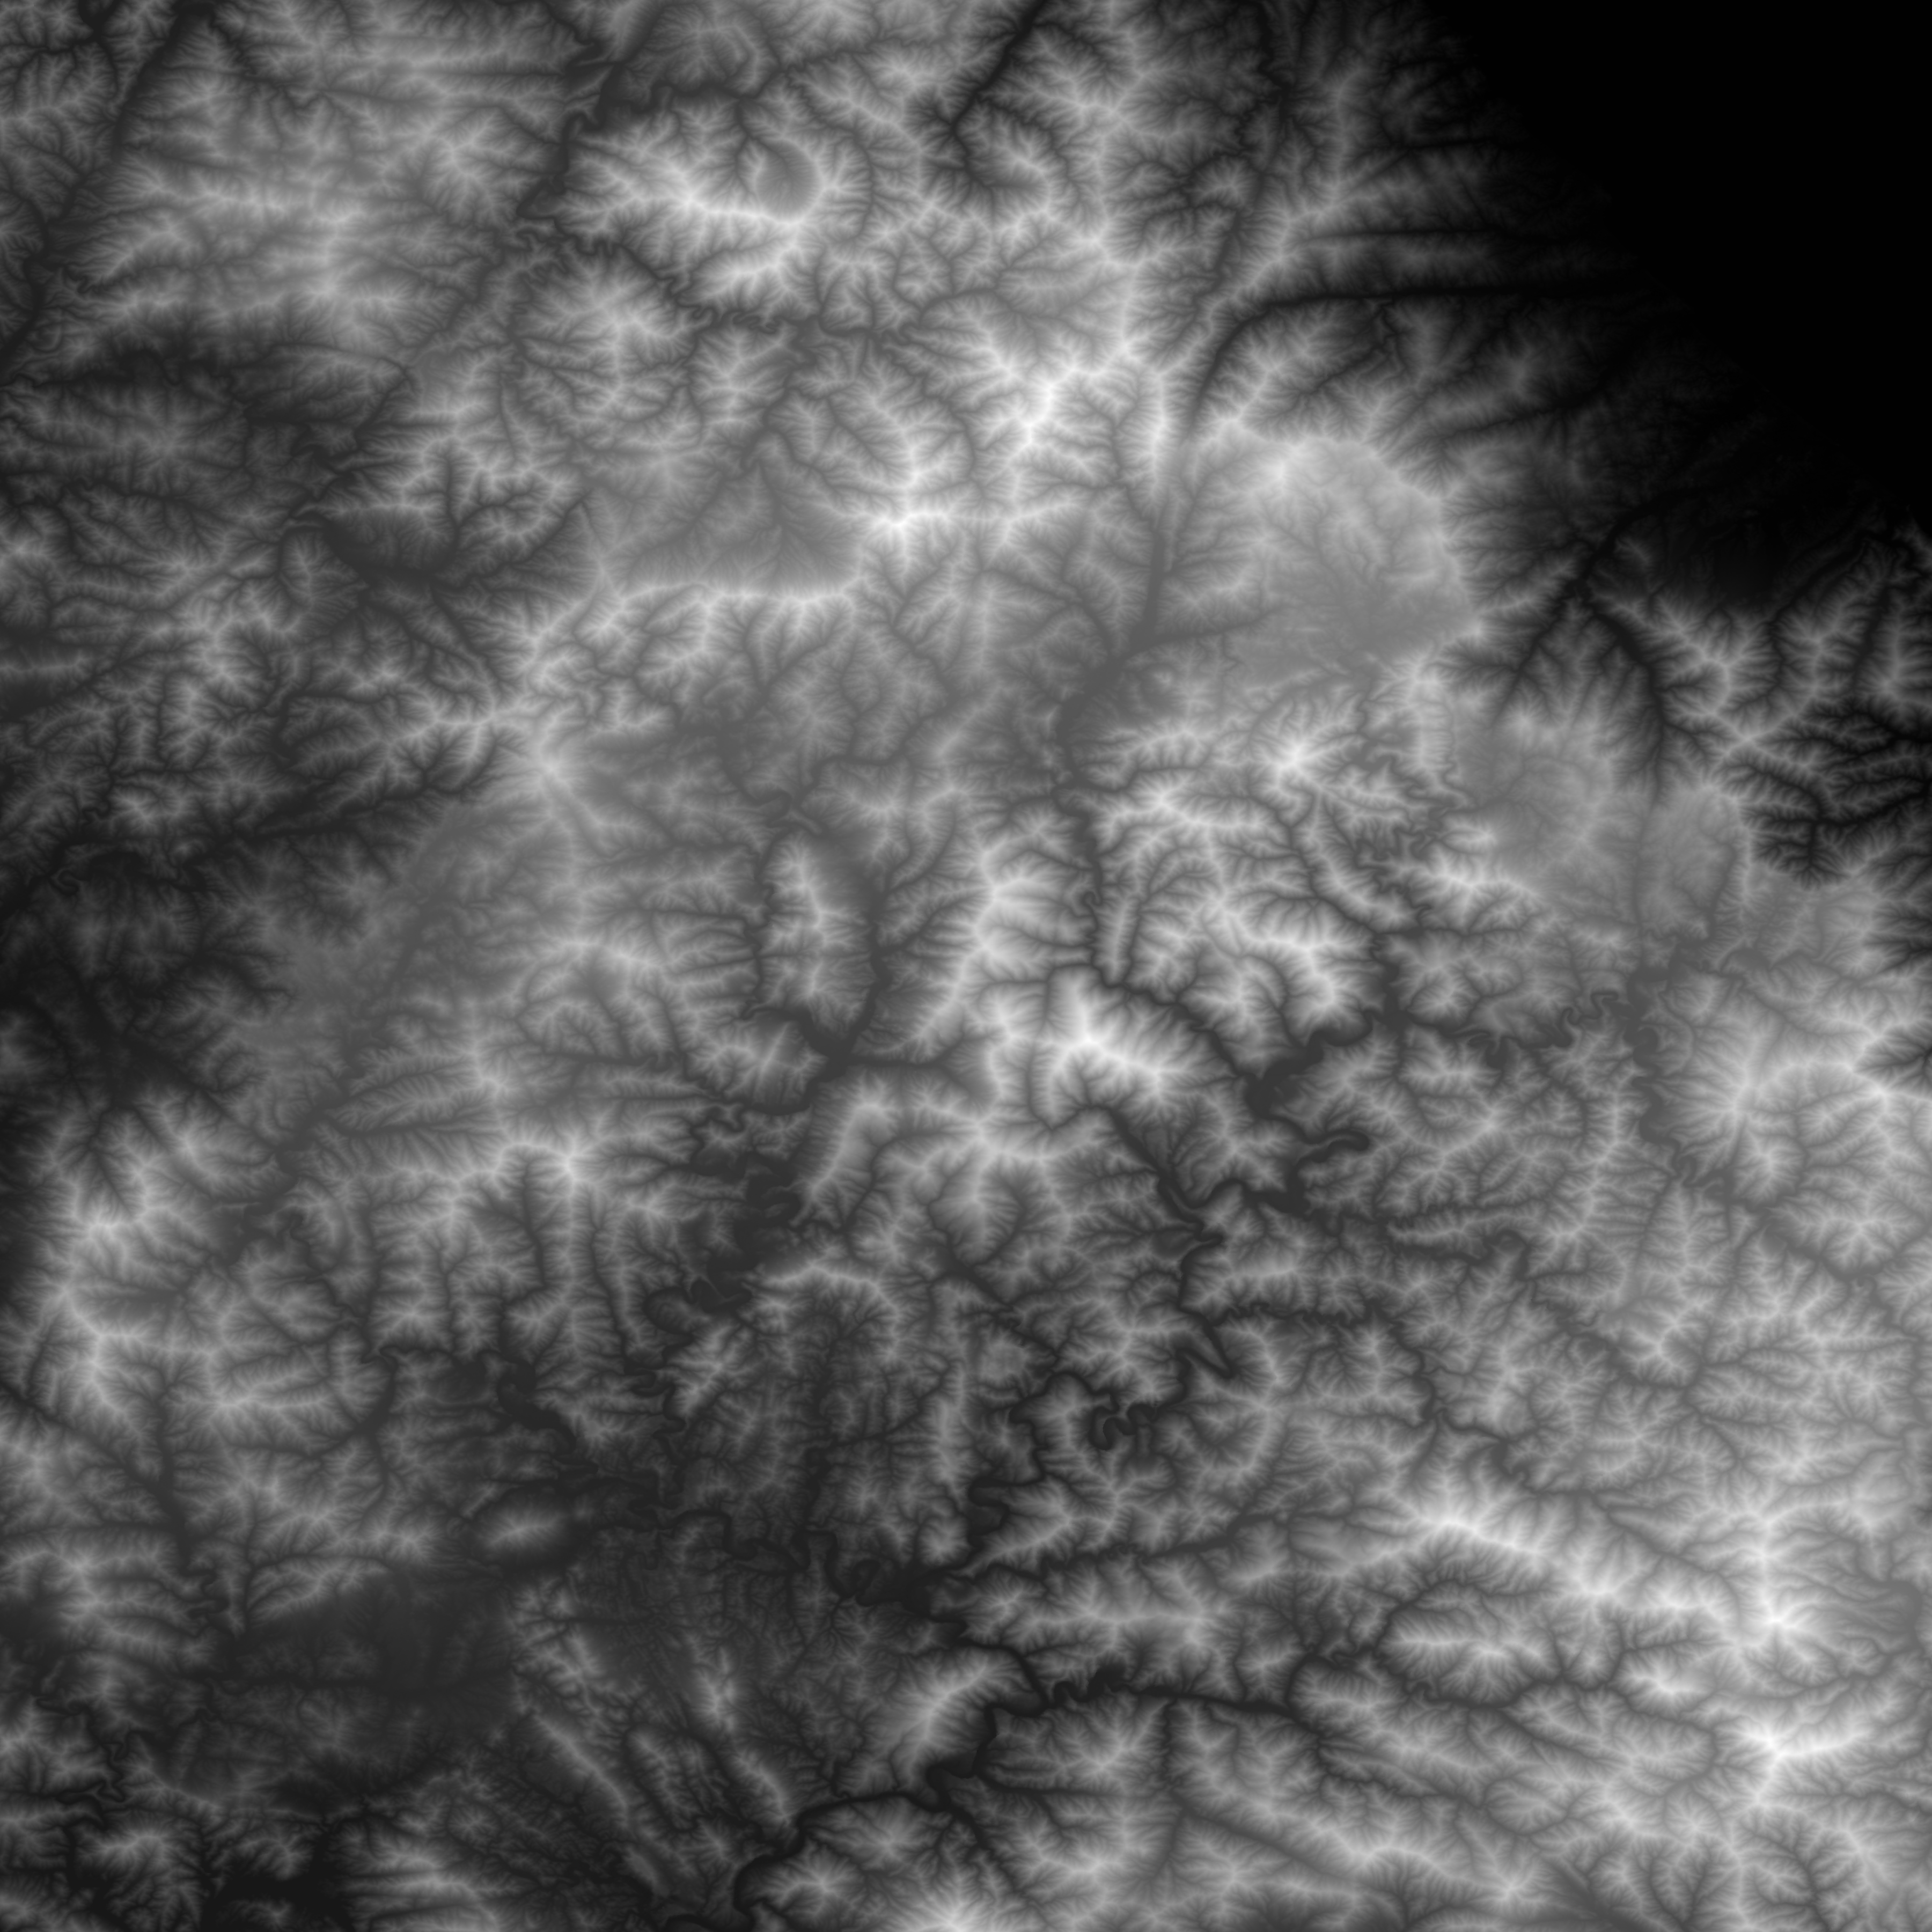
\includegraphics[trim=1cm 0.2cm 1.5cm 1.2cm, clip=true,scale = 0.05]{../figures/presentable_data/korea.png}
\caption[Taebbaek Mountain]{The Taebaek Mountain area in South Korea. The original image has a resolution of $3601\times 3601$ pixels. Downloaded from \url{https://earthexplorer.usgs.gov/} }\label{Korea}
\end{figure}
\section{Computational Implementation}
\subsection{Finding the ideal parameter $\lambda$}
In order to find the ideal parameter $\lambda$ for both LASSO and Ridge regression, we looped over a set of lambda-values in different magnitudes and estimated the MSE using 4-fold Cross Validation. We chose to use the parameter $\lambda$ that gave the lowest MSE, averaged over two uncorrelated runs. This was repeated for each fit, that is,  $\lambda$ was recalculated for each new Design Matrix X. This is because the ideal $\lambda$ value changes with model complexity.
\subsection{Error in LASSO-Regression}
As there is no way to find the parameters $\bm{\beta}$ for LASSO-Regression analytically, numerical methods need to be used. Here, we used Scikit-Learn \cite{scikit-learn} in order to solve the problem numerically. We have observed that the LASSO-method converges rather slowly. We observed that setting the tolerance to 0.01 lead to no convergence even at $10^5$ iterations at higher polynomial degrees when fitting the Franke Function. Having LASSO converge is very time-consuming, we found it impossible to run a large-scale numerical experiment with properly converging LASSO regression when the datasets are large, many polynomial degrees are to be included, and there a large number of bootstraps. For this reason, we have chosen the tolerance to be equal to 0.03 for fitting the Franke function, while the number of maximum iterations is chosen to be $10^5$.  Similarly, we used 0.3 as tolerance at $10^2$ maximum iterations for fitting the country data - this is not sufficient to get a proper fit.  Hence, each time the LASSO-fit was higher than the OLS fit, no ideal parameters have been found, as the ideal LASSO-fit cannot be no larger than the OLS-fit (because $\lambda=0$ is the OLS fit).
\subsection{Sampling Franke Function}
We sample randomly points $x_i$ and $y_i$ between 0 and 1 and calculate the target points
\begin{equation*}
z_i=f(x_i,y_i)+\epsilon_i
\end{equation*}
where $\epsilon_i$ follow a normal distribution with standard deviation $\sigma$. We used different values for $\sigma$, usually in the range $[0.01,1]$, which has a profound impact on the fit. 
\subsection{Sampling Image Data}
We sampled N randomly chosen points from the picture, where $N \in \{5000, 20000, 50000 \}$.
\subsection{The Design Matrix}
The Design Matrix implemented is a 2D-version of the Vandermonde Matrix, hence, approximate $z_i$ as, for a given degree $k$
\begin{equation*}
\tilde z_i=\beta_0+\beta_1x_i+\beta_2y_i+\beta_3x_i^2++\beta_2x_iy_i+...+\beta_py_i^k
\end{equation*}
In the practical implementation, we "drop" $\beta_0$ by removing the first column from the Design Matrix, as our data is scaled.
\subsection{Scaling}
The design matrix is scaled using Scikit-Learn's StandardScaler. While this is not necessarily necessary for OLS, scaling is needed in order to ascertain that Ridge regression \& LASSO regression scale parameters equally, giving an overall better result. 
\subsection{Test functions and reproducibility}
In order to ascertain the validity of our results, we implemented several test functions, where we tested that the Design Matrix is set up properly, that the functions performing the Regressions give the expected results, and that the main error estimates ($R^2$ \& MSE) are implemented correctly. \\
All data was created using the same random number seed, which can be found in the program files, hence our results should be reproducible by choosing identical parameters.
\subsection{Explanation of Code}
As stated in the Introduction, all data can be found on our \href{https://github.com/schraderSimon/FYS-STK/tree/master/project1}{Github address}. In the main folder, an explanation of the code can be found. How the code is to be executed, is stated in the bottom of each file.
\section{Results}

\subsection{$\beta$ standard deviation in OLS and Ridge regression}
Using OLS and Ridge regression, for a given polynomial degree, the radius of the 95'th percentile confidence interval of the parameter $\beta$ with the largest standard deviation was calculated and tabulated. The result is shown in table \ref{betaVarianceTable}.

\begin{table}[H]\caption[Confidence interval of estimators in OLS vs. Ridge]{Half the width of the 95'th percentile confidence interval for the estimators $\beta$ in OLS and Ridge regression with the highest standard deviation, using the regularization parameter $\lambda$. }
\label{betaVarianceTable}
\begin{tabular}{|r|r|r|r|}
\hline
polynomial degree & OLS   & Ridge ($\lambda = 0.1$) & Ridge ($\lambda = 1.0$) \\ \hline
1                 & 0.005 & 0.014                & 0.013          \\
2                 & 0.023 & 0.062                & 0.047          \\
3                 & 0.128 & 0.207                & 0.077          \\
4                 & 0.632 & 0.250                & 0.086          \\
5                 & 2.977 & 0.278                & 0.091 \\ \hline
\end{tabular}
\end{table}
It's clear that Ridge regression has the effect of tightening the confidence interval for the parameters $\beta$ belonging to the highest order polynomials. It's also clear that increasing the regularization parameter $\lambda$ has the expected effect of further tightening the confidence interval of the parameters. It's worth noting that while in OLS the values occupy four different orders of magnitude, but using Ridge, that decreases to two or one. The cost function imposing a penalty on the size of the $\beta$'s, forces every parameter to within a smaller subset of options.\\\\ For the same analysis on the terrain data, we got the results in table \ref{table2}.



\begin{table}[H]\caption[Confidence intervals of estimators in OLS and Ridge regression for Geodata]{The column names  are abbreviated as: p.d.- Polynomial degree, C.I (Confidence Interval), meaning here, half the width of the 95'th percentile confidence interval for the estimators $\beta$ in OLS and Ridge regression with the highest standard deviation, using the regularization parameter $\lambda$ found in the parentheses. $b_{min/max}$ the lowest and highest value of $\beta$ used in the model}
	\begin{adjustbox}{max width=\textwidth}
		\csvautotabular{../csvData/g_confidence_intervals_maxdeg_15.csv}
	\end{adjustbox}	
	\label{table2}
\end{table}

Here too, wee see that the implementation of ridge regression results in much lower variance in the parameters $\beta$ while also reducing the maximal parameters by many orders of magnitude .




\subsection{Error comparison}
\subsubsection{Bootstrap vs. Cross validation}
Bootstrap and K- fold cross validation is here used to estimate the error in our models. We're evaluating the error estimation of Bootstrap and K- fold cross validation in terms of MSE on the same dataset using a fixed value for $\sigma$, a fixed number of data points and fixed model complexity. The objective being to compare the two resampling methods, varying only the amount of folds used in K- fold cross validation. Using a dataset constructed from the Franke function, we get figure \ref{BootstrapVsKfold1}.

\begin{figure}[H]
\centering

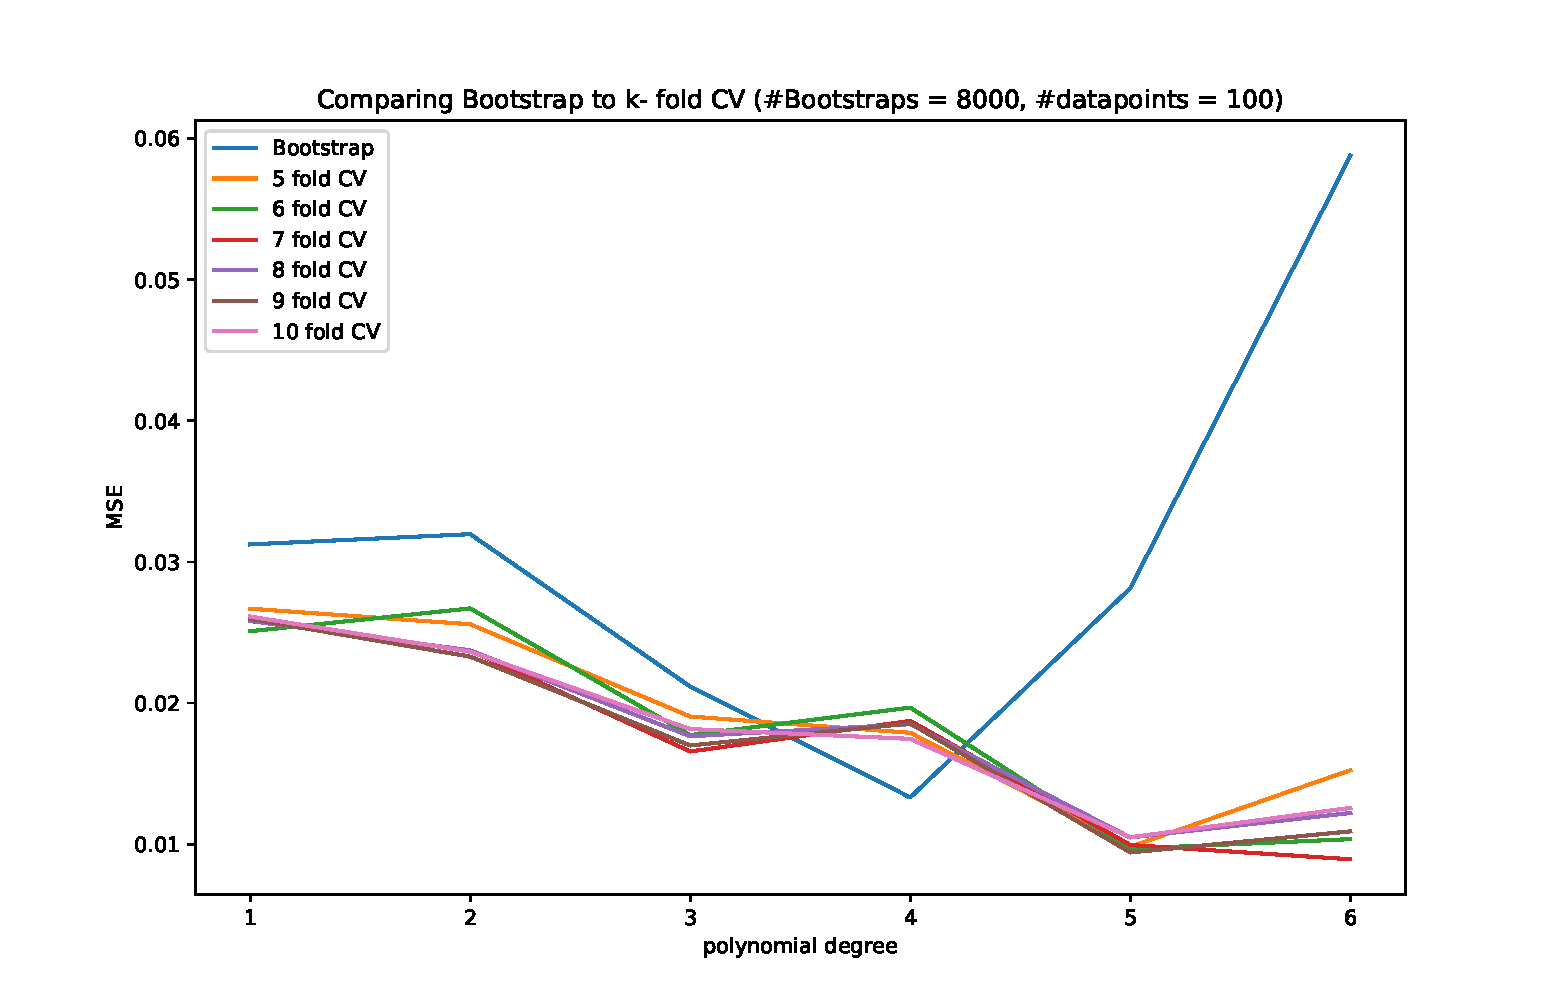
\includegraphics[trim=1.4cm 0.2cm 2.5cm 1.2cm, clip=true,scale = 0.5]{KfoldVsBootstrap_k5to10_8kBootstraps.pdf}
\caption[Comparing Error estimates from Bootstrap vs. K- fold CV]{Estimated MSE as a function of model complexity (polynomial degree) for different values of $k$, using k- fold CV and Bootstrap OLS on the Franke function \eqref{FrankeFunction}. We see that all iterations of K- fold cross validation makes a lower error estimate than 8000 bootstraps on this very limited data set of 100 entries}\label{BootstrapVsKfold1}
\end{figure}
Trying again, this time with 10 times as many data points. We get figure \ref{BootstrapVsKfold2}

\begin{figure}[H]
\centering

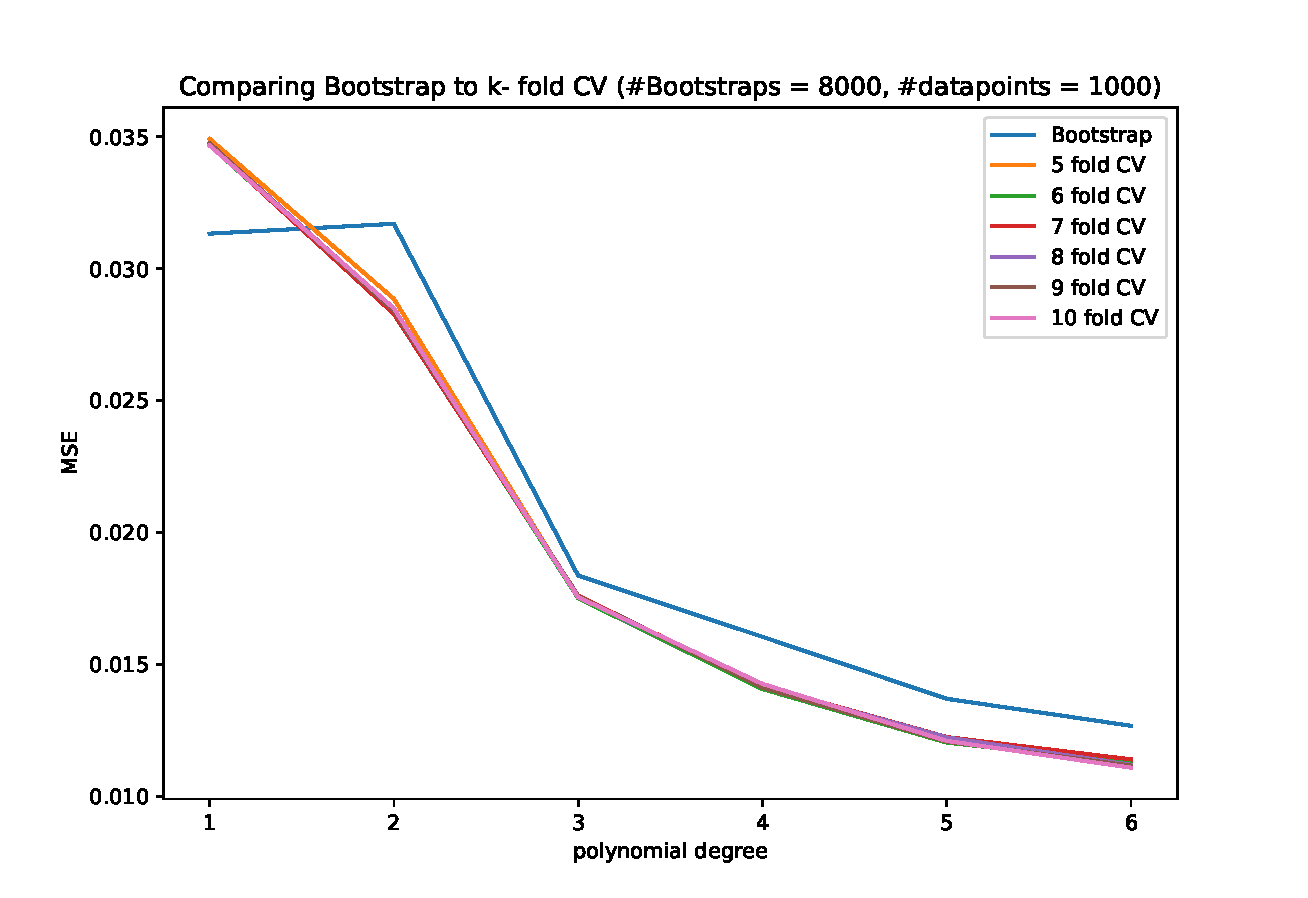
\includegraphics[trim=1cm 0.2cm 1.5cm 1.2cm, clip=true,scale = 0.6]{KfoldVsBootstrap_k5to10_8kBootstraps_1000dps.pdf}
\caption[Comparing Error estimates from Bootstrap vs. K- fold CV -1000 data points]{Estimated MSE as a function of model complexity (polynomial degree) for different values of $k$, using k- fold CV and Bootstrap OLS on the Franke function \eqref{FrankeFunction}. Again, all iterations of K- fold cross validation makes a lower error estimate than 8000 bootstraps. However, increasing the number of data points made the difference significantly smaller, especially for the more complex models.}\label{BootstrapVsKfold2}
\end{figure}
Figures \ref{BootstrapVsKfold1} and \ref{BootstrapVsKfold2} give the impression that on a sufficiently large dataset, Bootstrap gives comparable error estimates with K- fold cross validation. Bootstrap, however comes at a significantly higher computational cost which we've yet to show explicitly.\\Using the same model as above, we run K- fold cross validation with $k=10$ and compare the elapsed time with Bootstrap. The result is shown in figure \ref{BootstrapVsKfold3}.

\begin{figure}[H]
\centering

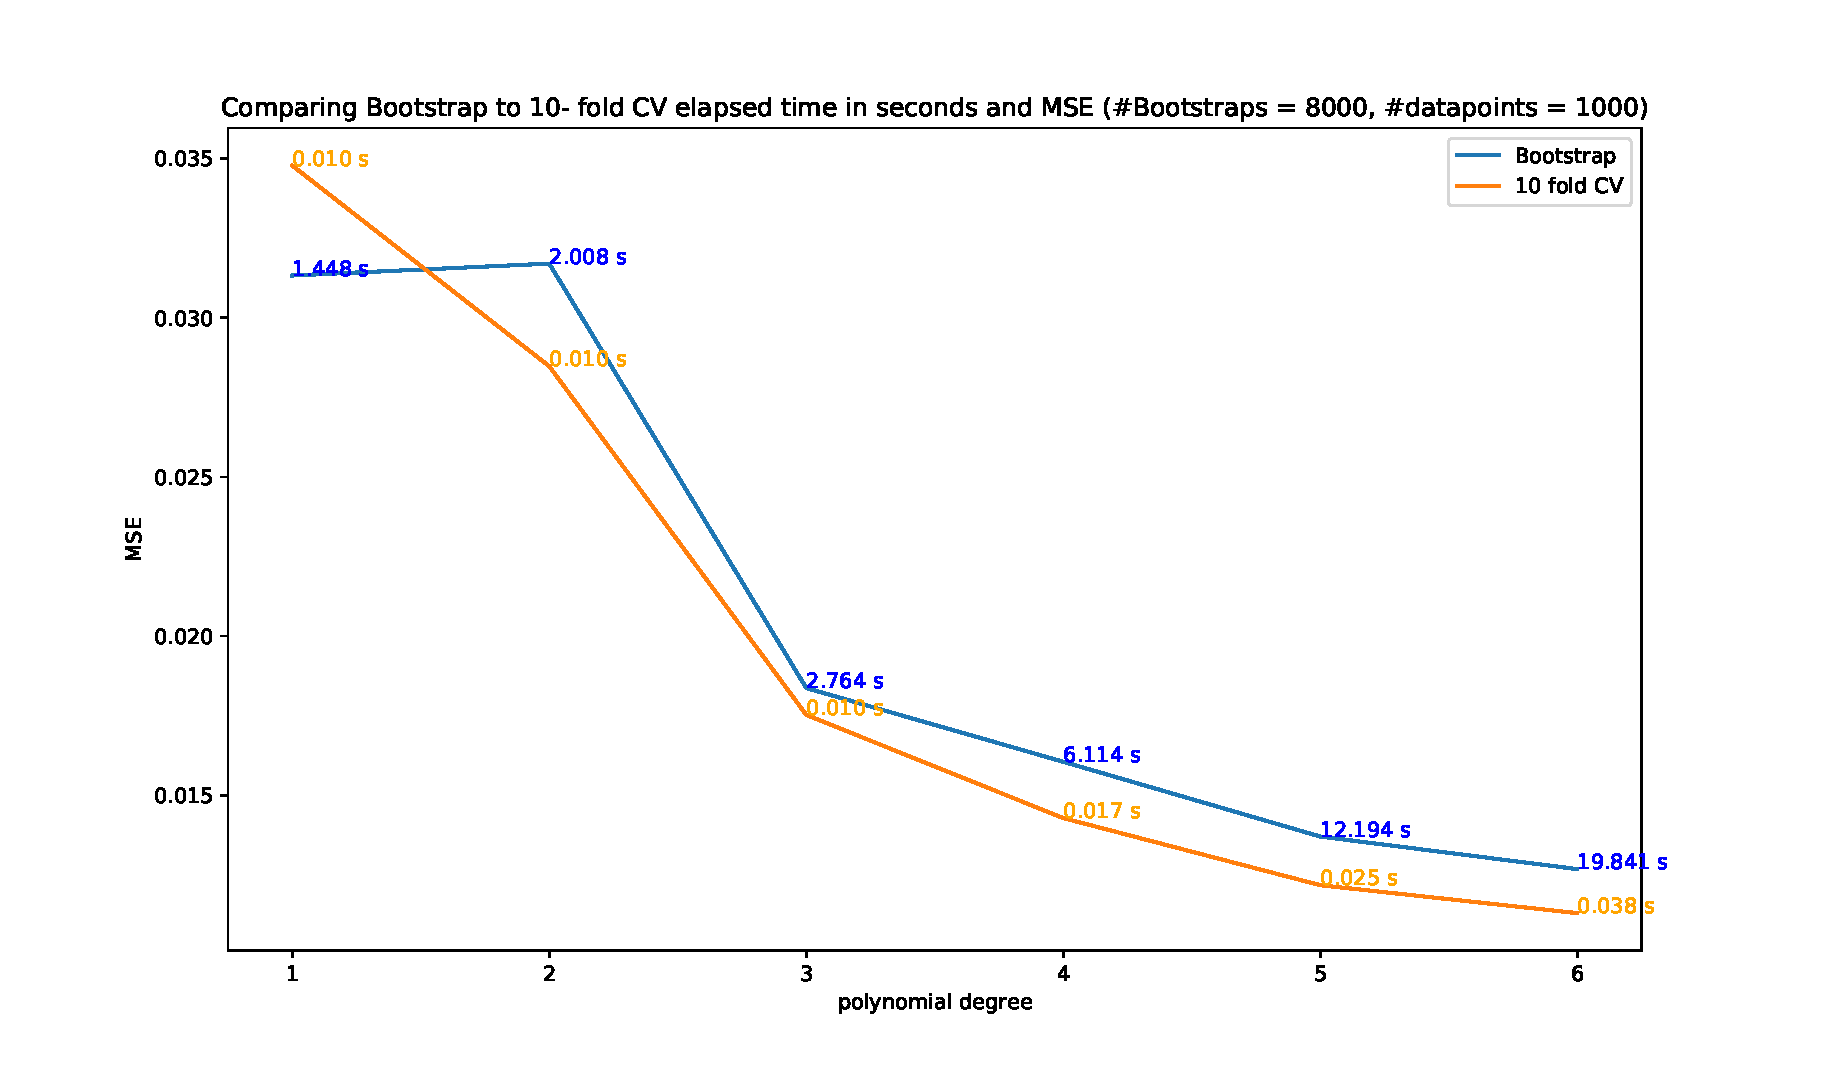
\includegraphics[trim=2.0cm 0.9cm 2.7cm 1.2cm, clip=true,scale = 0.5]{KfoldVsBootstrap_k10_8kBootstraps_elapsedTime_comparison.pdf}
\caption[Comparing time elapsed from Bootstrap vs. K- fold CV]{Estimated MSE as a function of model complexity for $k=10$, using k- fold CV and Bootstrap OLS on the Franke function \eqref{FrankeFunction}. The time elapsed for each model is plotted. Not only does K- fold CV take considerably less time, but the time increases much slower with increased model complexity compared to Bootstrap.}\label{BootstrapVsKfold3}
\end{figure}


\subsubsection{Franke Function}
Using resampling methods, the MSE for OLS, Ridge- and LASSO regression on the Franke function were plotted against the model complexity.
\begin{figure}[H]
\centering
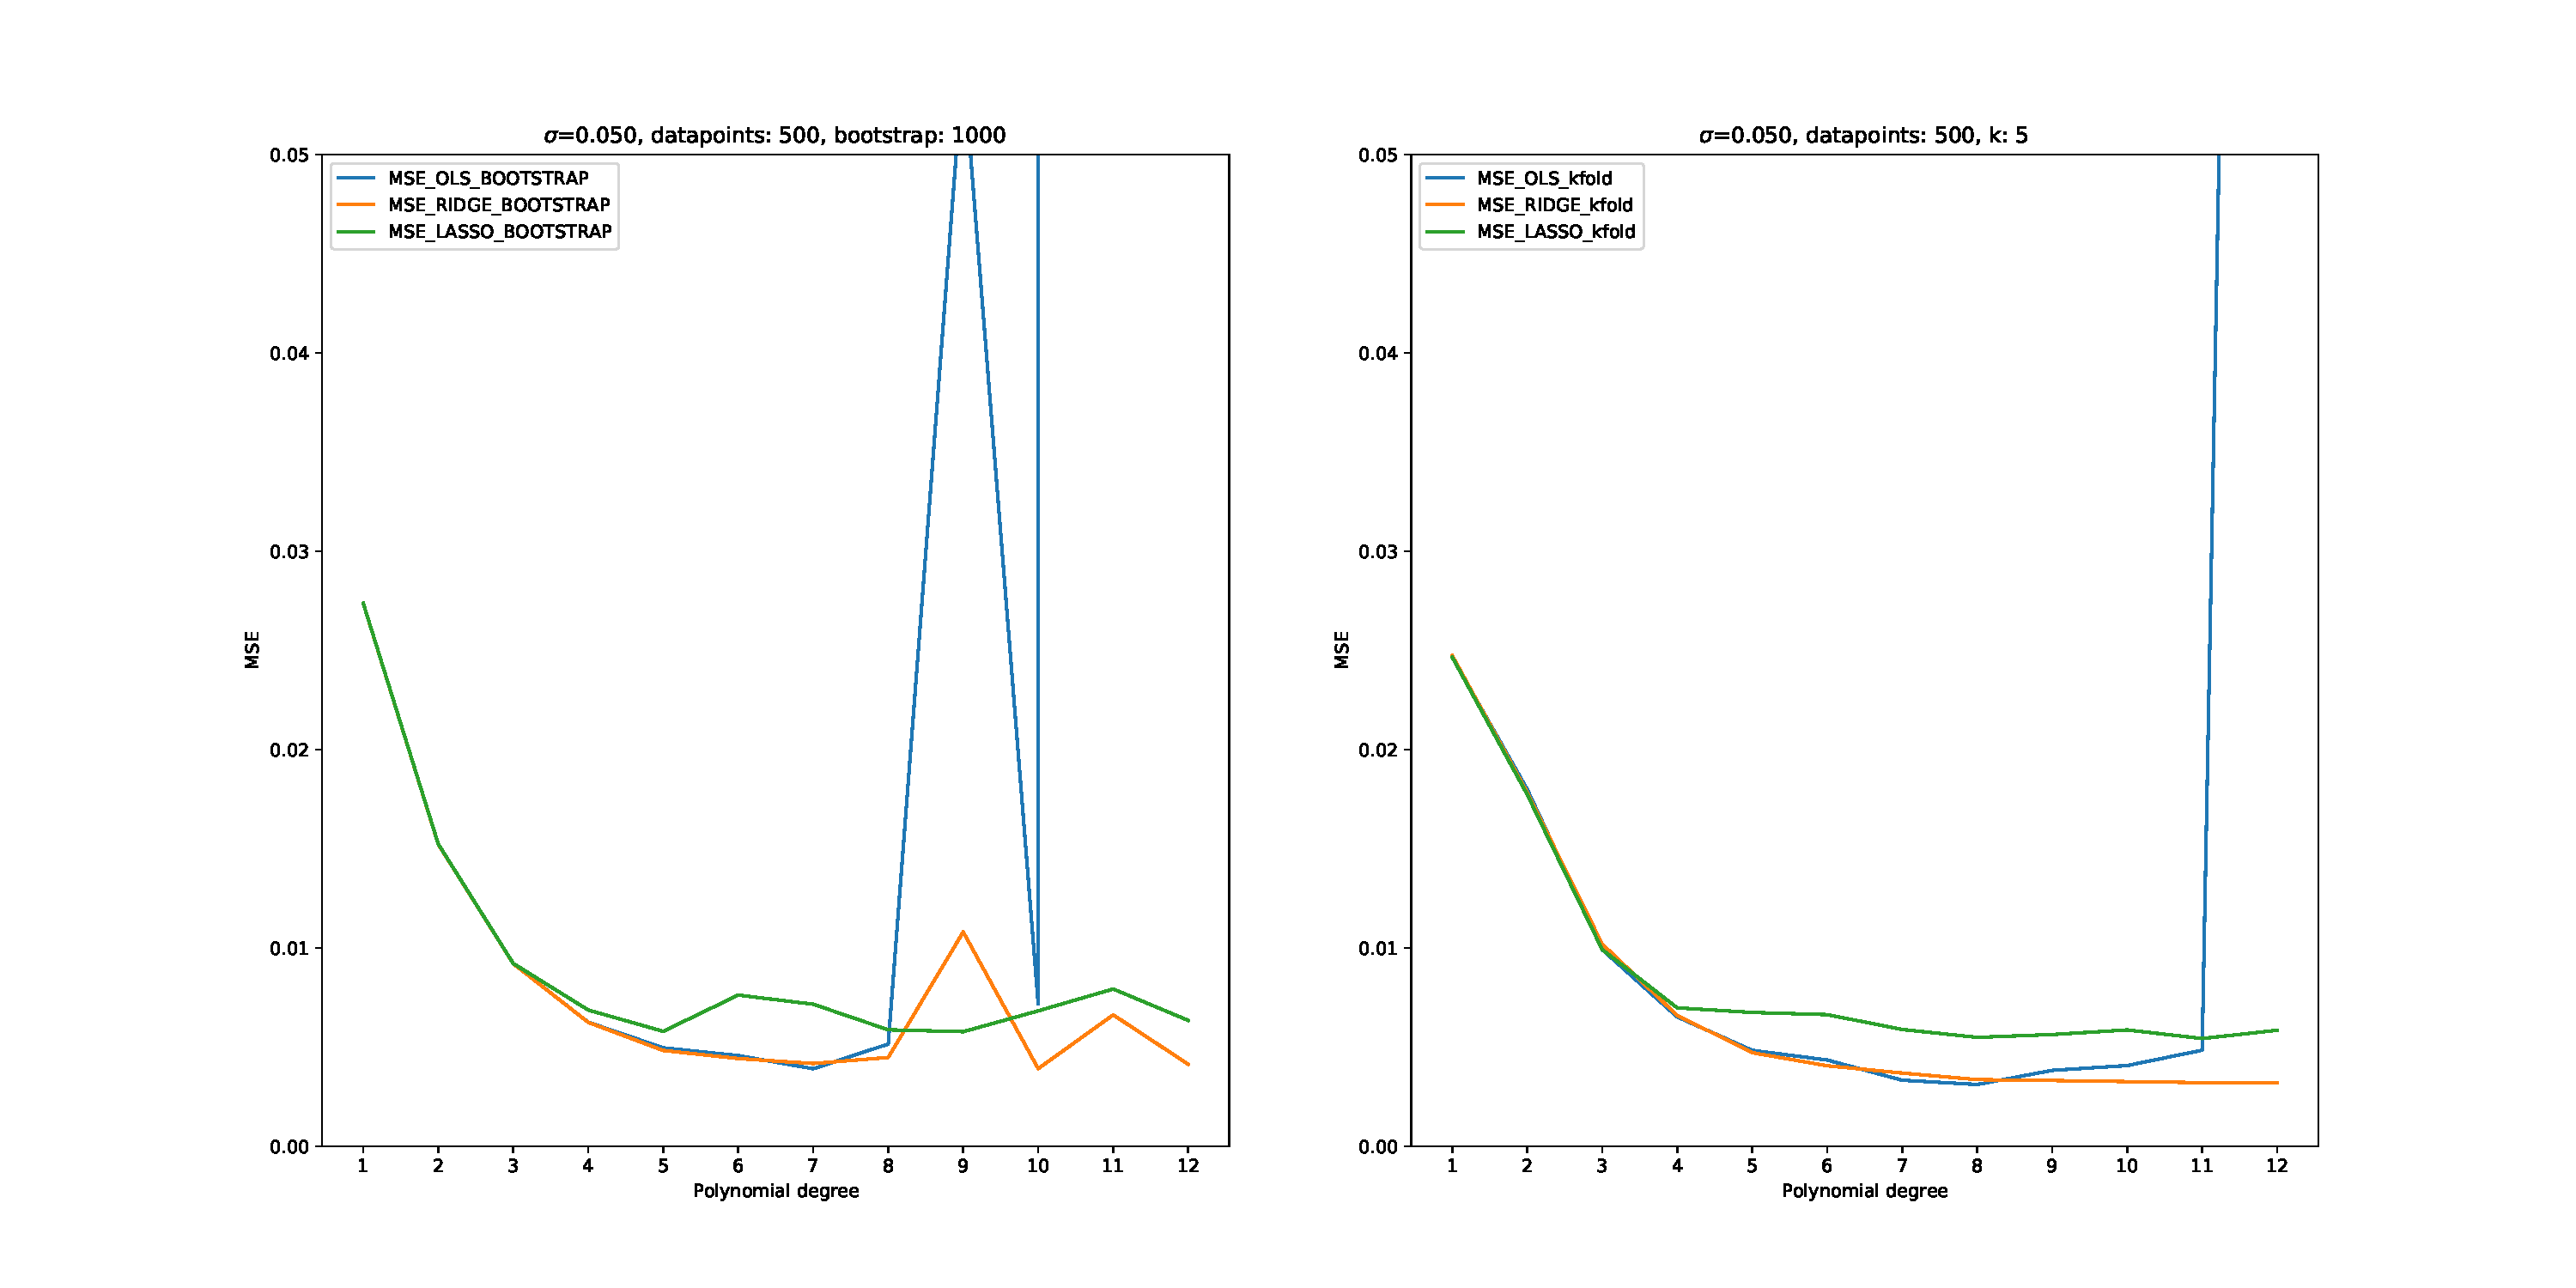
\includegraphics[width=0.95\textwidth]{MSE_different_methods_Franke.pdf}
\caption[Test MSE for LASSO, Rigde and OLS regression (Franke)]{Test MSE for LASSO, Rigde and OLS regression. Estimated using Bootstrap (left) or k-Fold Cross validations. The exact parameters can be found in the graph's title. Here, LASSO does not converge.}
\label{fig:MSE_different_methods_Franke}
\end{figure}
\begin{figure}[H]
\centering
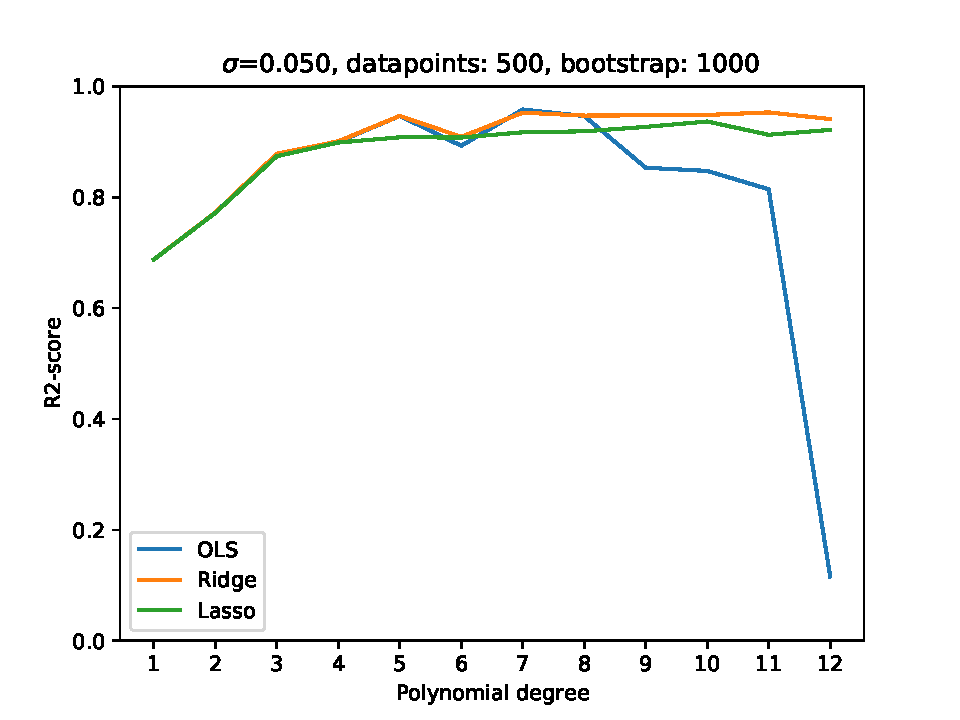
\includegraphics[trim=0.7cm 0.2cm 1cm 0.85cm, clip=true,scale = 0.7]{R2_bootstrap_different_methods_Franke.pdf}
\caption[Test $R^2$-value for LASSO, Rigde and OLS regression]{Test $R^2$-value for LASSO, Rigde and OLS regression. Estimated using Bootstrap (left) or k-Fold Cross validations. The exact parameters can be found in the graph's title. The LASSO method did not converge here.}
\label{fig:R2_different_methods_Franke}
\end{figure}

As expected from the theory, increasing the model complexity lead to a decreased Mean-Square-Error and an increased $R^2$ score for all three methods when fitting the Franke Function. However, as can be seen in figures \ref{fig:MSE_different_methods_Franke} and \ref{fig:R2_different_methods_Franke}, the mean square error for the Ordinary Least Square approximation suddenly raises sharply (and the $R^2$ score drops sharply) after some complexity is reached: This behaviour cannot be observed with LASSO and Ridge. Neither LASSO nor Ridge give conceivably better results than OLS when looking at the complexity giving the best results, that is, with the chosen parameters, OLS, LASSO and Ridge regression are about equally fast. As OLS is the most basic method, easiest to implement and also fastest, we figured out that it is the most suitable method for this problem - adding more complexity while avoiding a high variance (Ridge or LASSO) does not improve the quality of the fit.  Another interesting observation is that there is much more fluctuation in the MSE when using bootstrap than when using 5-fold Cross validation. We are not quite sure why this happens, but we assume that one possible cause is that when using bootstrap, some very "undesirable" combinations of values might be chosen, which leads to a very high Bootstrap. Thus, the graphs might look smoother when running more Bootstrap-samples. Another reason is that the training set in the Bootstrap method is not equally large as the training set when using 5-fold cross validation (75\% vs 80\%). We also observed that Bootstrap is more time-demanding than k-fold Cross Validation. As Bootstrap and Cross Validation are two very different methods to estimating a value of interest, the MSE in this case, different results are not surprising anyways. It would however be troublesome if the two methods gave different "ideal" models. The large deviation between LASSO and OLS is due to the aforementioned error. \\
We also ran a small simulation where LASSO regression does converge. This can be found in figure \ref{fig:ConvergingLasso_Franke}. From this graph, we see that LASSO behaves similarly to Ridge regression - the error does remain low even when the OLS regression MSE raises sharply. The LASSO fit is sometimes above the OLS fit, which means that the ideal parameter $\lambda$ for LASSO-regression has not been found. It is also interesting to see that Cross-Validation attributes finds a sharp "rise" in Ridge regression at degree 5, while LASSO regression doesn't have that.
\begin{figure}[H]
\centering
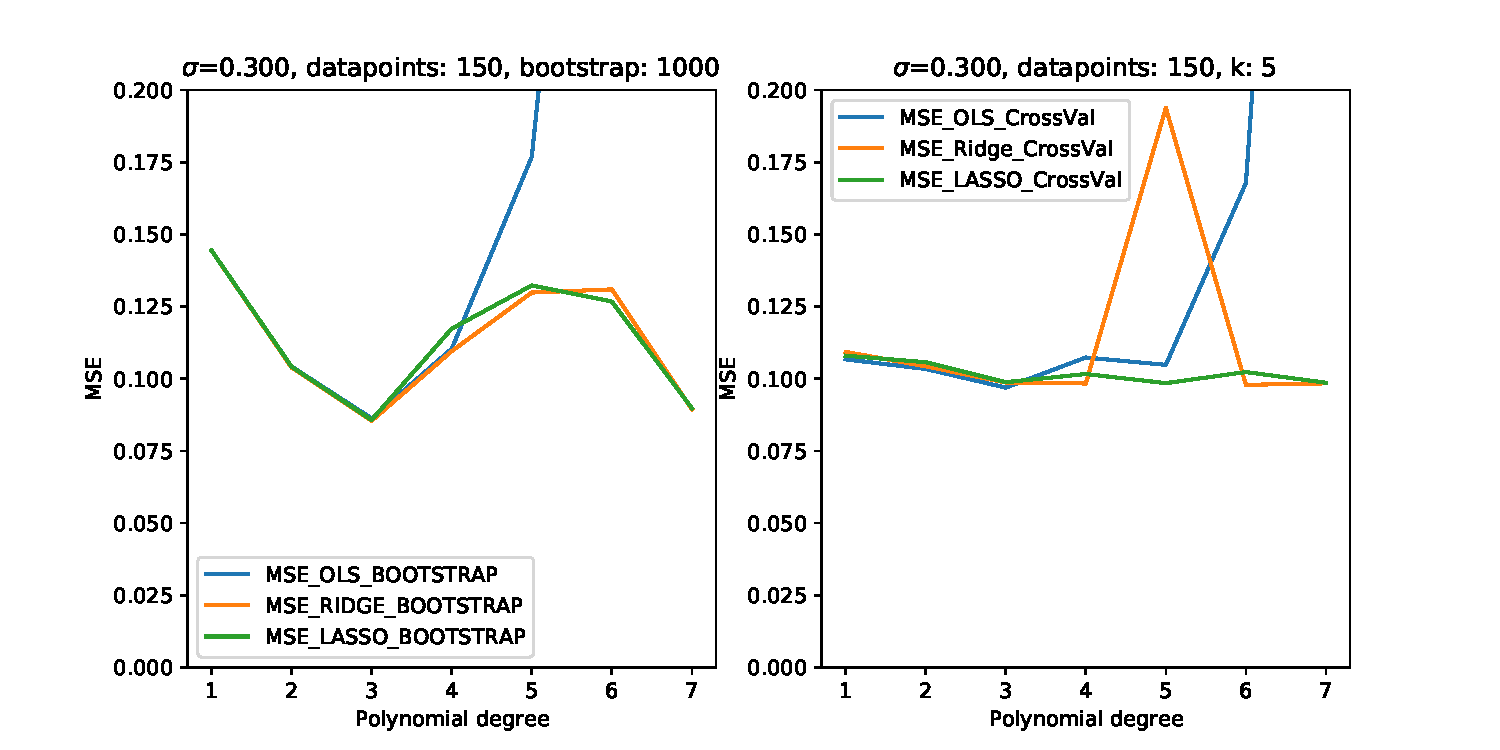
\includegraphics[width=0.95\textwidth]{MSE_different_methods_Franke_small.pdf}
\caption[Test MSE for LASSO, Rigde and OLS regression (Franke, small)]{Test MSE for LASSO, Rigde and OLS regression. Estimated using Bootstrap (left) or k-Fold Cross validations. The exact parameters can be found in the graph's title. Here, LASSO does converge.}
\label{fig:ConvergingLasso_Franke}
\end{figure}

\subsubsection{Geographic Data}
Figure \ref{fig:MSE_Korea} shows the Mean Square Error of fitting the geographic data as a function of polynomial degree for both Bootstrap and K-Fold Cross Validation for all three methods. We have chosen a value $\lambda$ which minimizes the MSE. 
\begin{figure}[H]
\centering
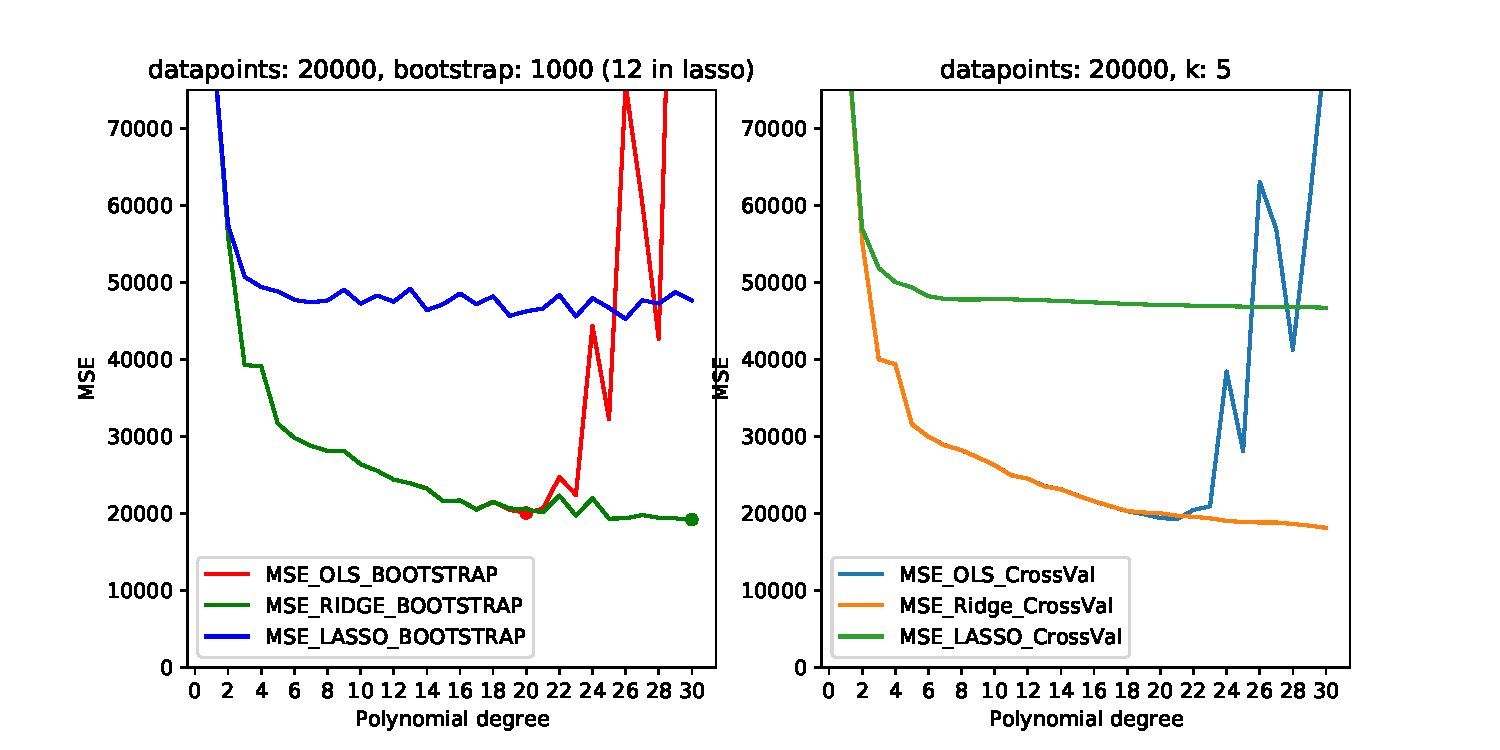
\includegraphics[width=0.95\textwidth]{MSE_different_methods_Korea_LARGE.pdf}
\caption[Test MSE for LASSO, Rigde and OLS regression (geo, 20000 points)]{Test MSE for LASSO, Rigde and OLS regression. Estimated using Bootstrap (left) or k-Fold Cross validations. The exact parameters can be found in the graph's title. LASSO regression did not converge.}
\label{fig:MSE_Korea}
\end{figure}
We found out that, using Bootstrap to estimate, the minimal MSE for both OLS and Ridge is around 20,000, slightly lower for Ridge with 19,000. Using 5-fold Cross Validation, we found the error to be 19,000 for OLS and 18,000 for Ridge-Regression. It is possible that the Ridge error might go down even more as the minimum occurs at the final degree(=30) we have included. We did not include higher polynomial degrees as this is computationally very expensive. The data looks similar to the data attained when fitting the Franke Function, just in a different magnitude of error: The error decreases sharply as the model complexity is increased, remains rather constant (or increases slowly) as it is increased more, and then raises again, sharply for OLS. The LASSO data is unreliable, as we have chosen to only include it for completeness reasons - we did not manage to reach a sufficiently converged value, hence the MSE is much larger than the minimal possible LASSO data.\\
We also run a second simulation with only 5000 datapoints. There, the minimal MSE was found to be around 23,000 for both OLS and Ridge using Bootstrap. From this, we assume that it is possible to attain even more precise fits with more fits, however, having the MSE reduced by 15\% while taking 4 times as many data points, is not impressive. We also run a third simulation with 50.000 data points. There, we used Cross-validation for the error estimate in order to reduce time usage. The result can be seen in figure \ref{fig:MSE_Korea_XXL}. The reason why we stopped at polynomial degree 40 and didn't try reducing the Ridge regression MSE further, is that higher polynomial degrees led to numerical overflow. Here, we got a minimal MSE of 16,500 for Ridge regression and 18,000 using OLS regression. This difference shows that Ridge regression can perform substantially better than OLS regression, but it also shows that the error reduction rate is really slow.
\begin{figure}[H]
\centering
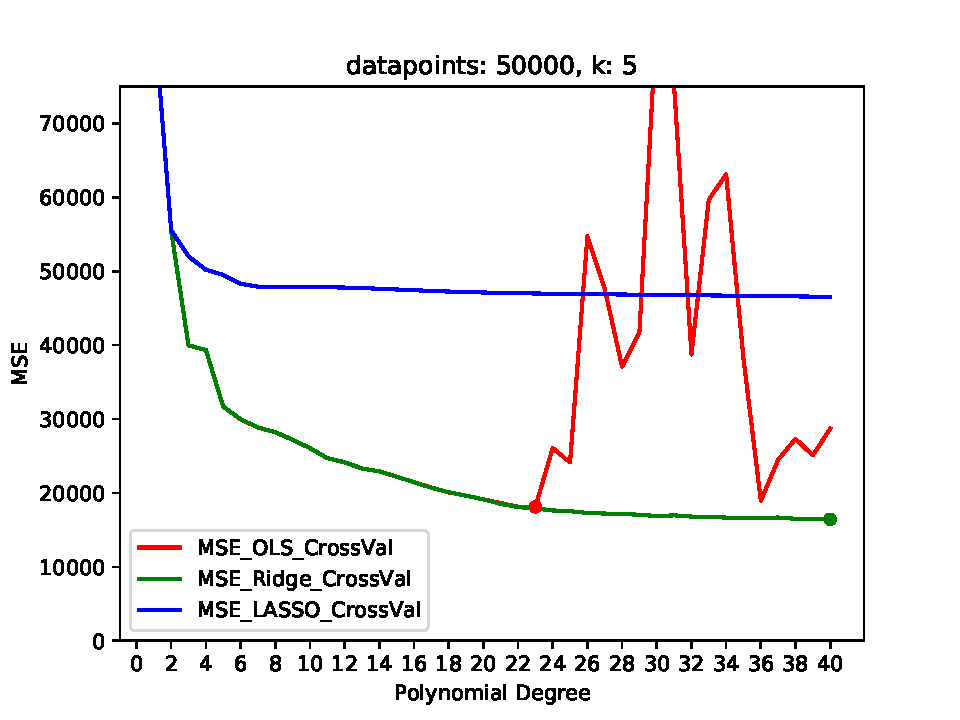
\includegraphics[width=0.65\textwidth]{MSE_different_methods_Korea50000_NOBOOTSTRAP.pdf}
\caption[Test MSE for LASSO, Rigde and OLS regression (geo, 50000 points)]{Test MSE for LASSO, Rigde and OLS regression. Estimated using 5-Fold Cross validations. The exact parameters can be found in the graph's title. LASSO regression did not converge.}
\label{fig:MSE_Korea_XXL}
\end{figure}

\subsection{Bias-Variance tradeoff}
\subsubsection{Franke Function}
\begin{figure}[H]
\centering
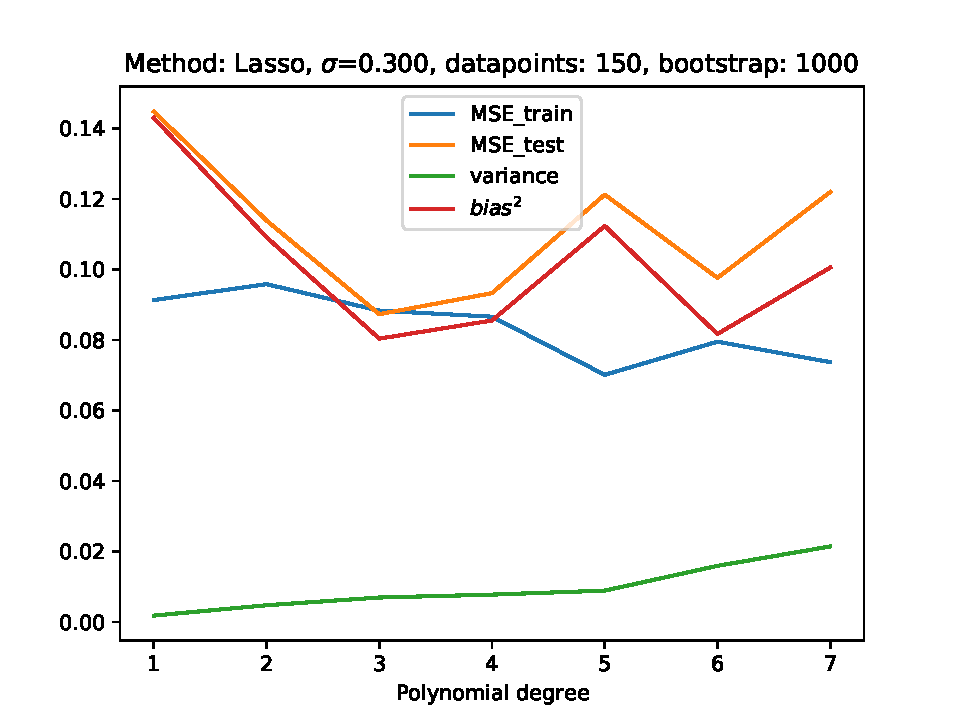
\includegraphics[width=0.65\textwidth]{Bias_Variance_LASSO.pdf}
\caption[Bias, Variance, MSE \& training MSE as a function of the polynomial degree using LASSO regression]{Bias, Variance, MSE \& training MSE as a function of the polynomial degree using LASSO regression. The values for $\sigma$, the size of the dataset and the number of bootstraps can be found in the title. Here, the LASSO method converges.}
\label{fig:LASSO_Bias_Variance}
\end{figure}
\begin{figure}[H]
\centering
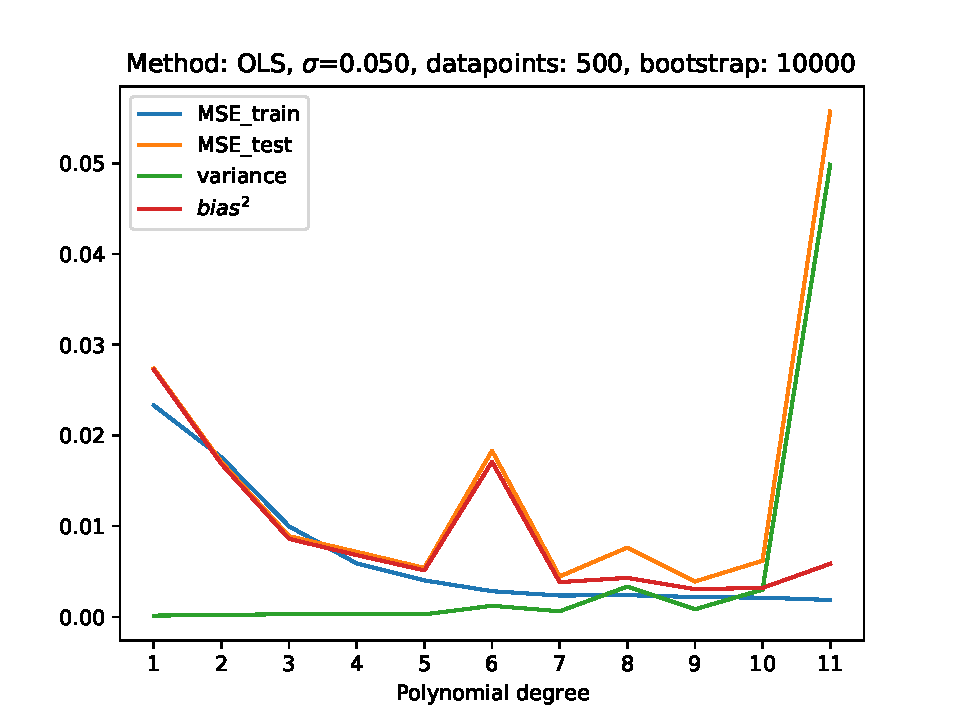
\includegraphics[width=0.65\textwidth]{Bias_Variance_OLS.pdf}
\caption[Bias, Variance, MSE \& training MSE as a function of the polynomial degree using OLS regression]{Bias, Variance, MSE \& training MSE as a function of the polynomial degree using OLS regression. The values for $\sigma$, the size of the dataset and the number of bootstraps can be found in the title.}
\label{fig:Bias_Variance}
\end{figure}
\begin{figure}[H]
\centering
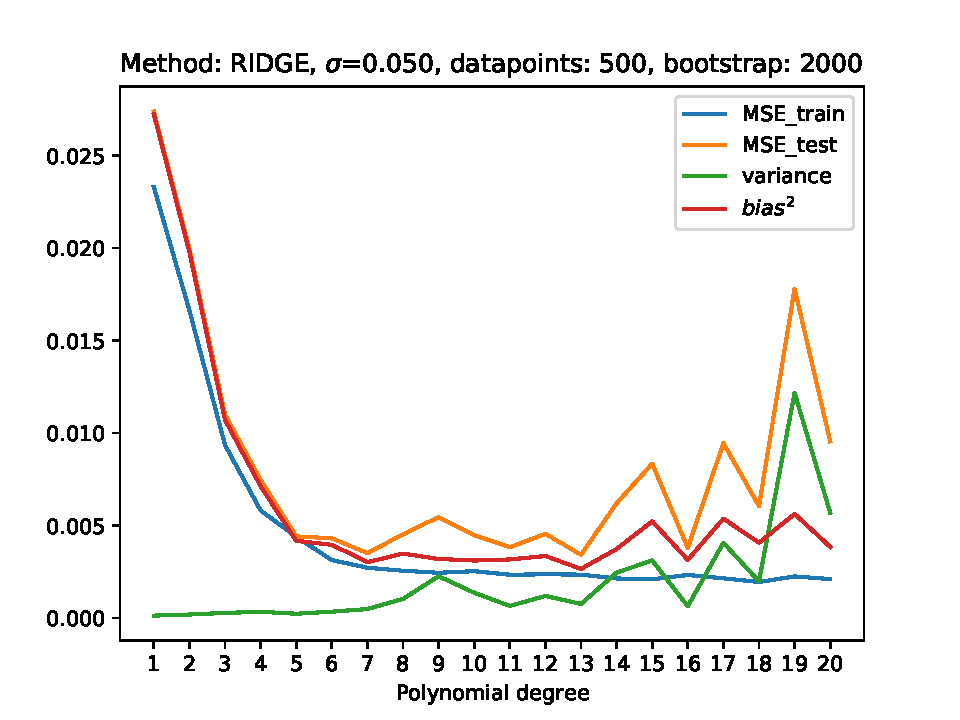
\includegraphics[width=0.65\textwidth]{Bias_Variance_RIDGE.pdf}
\caption[Bias, Variance, MSE \& training MSE as a function of the polynomial degree using Ridge regression]{Bias, Variance, MSE \& training MSE as a function of the polynomial degree using Ridge regression. The values for $\sigma$, the size of the dataset and the number of bootstraps can be found in the title.}
\label{fig:Ridge_Bias_Variance}
\end{figure}
Figures \ref{fig:LASSO_Bias_Variance}, \ref{fig:Bias_Variance} and \ref{fig:Ridge_Bias_Variance} show the MSE, the Training-MSE, the Variance, and the bias for the Franke Function. We chose a very small set for the LASSO regression where the results converge properly, so this cannot be compared to the other sets directly. However, figure \ref{fig:ConvergingLasso_Franke} contains the MSE for OLS and LASSO as well that was created with the same data. In all figures, the aforementioned statement that the variance increases and the bias decreases with increasing model complexity, hold true. Especially for the OLS, we see that this resembles  figure 2.11 on page 38 in \citep{hastie01statisticallearning} a lot. One can see that OLS is more prone to a higher variance at higher polynomial degrees, as is expected - shrinkage methods explicitly reduce the variance. \\However, we have also observed that the test MSE does not form a nice "U"-shape, but that both the bias and the variance can be quite "whacky" and do large jumps. That the bias goes up and the variance goes up as the complexity increases, remains a general trend, however, the variance does sometimes decrease at higher complexities, while the bias increases. We see that for Ridge regression in figure \ref{fig:Ridge_Bias_Variance}. This happens even when performing 10,000 bootstrap samples. The shape depends on several factors, among them the random number seed, the number of bootstraps, the number of data points as well as the chosen standard deviation from the "true" Franke function. Examples of this can be found in the appendix (figure \ref{fig:Bias_Variance_fucked}).
\subsubsection{Geographic Data}

Figure \ref{fig:biasVariance_Korea} shows the bias, the variance and the MSE as a function of polynomial degree for Ridge and OLS regression. We have chosen a value $\lambda$ which minimizes the MSE. We decided not to include LASSO as the LASSO data we attained is not the true LASSO data.
\begin{figure}[H]
\centering
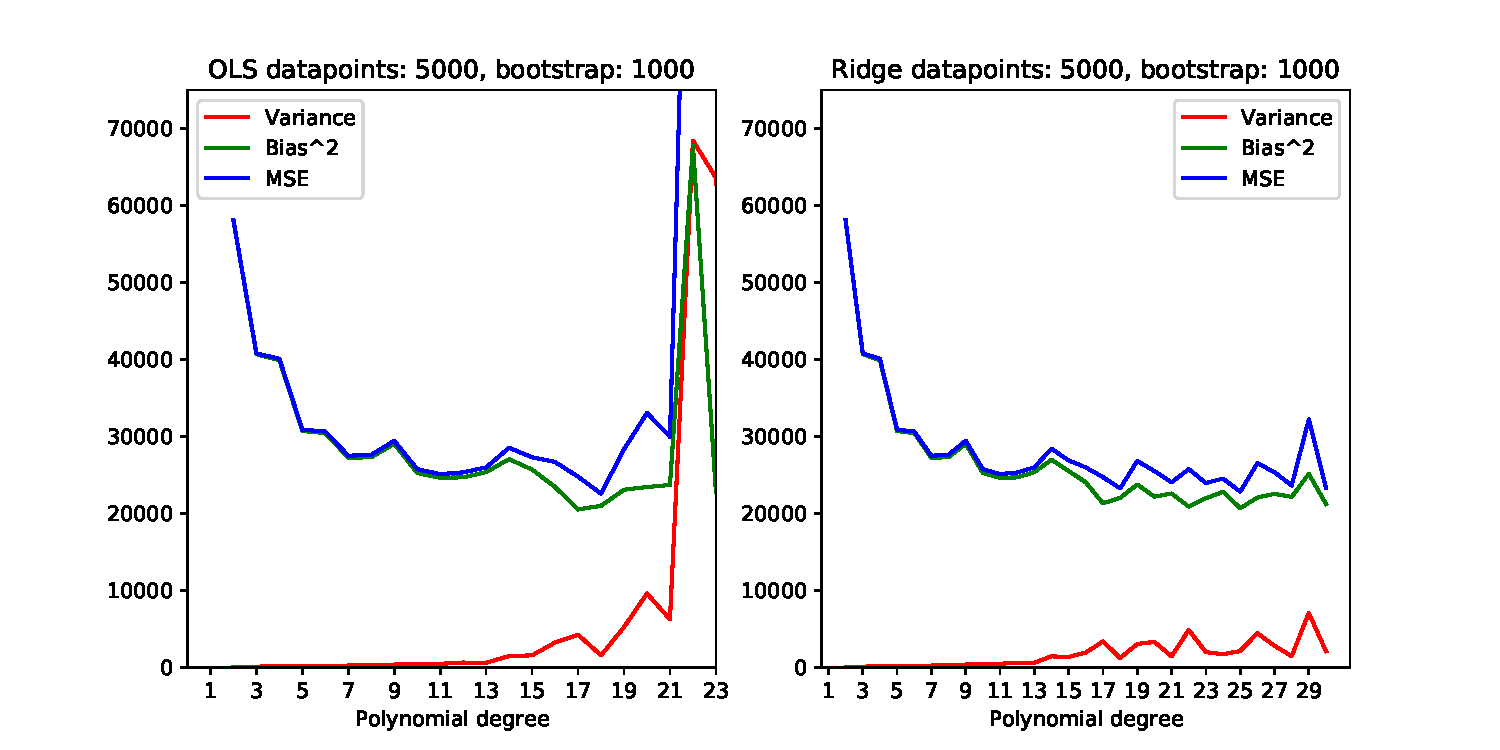
\includegraphics[width=0.95\textwidth]{Bias_variance_Korea.pdf}
\caption[Bias, Variance, MSE \& training MSE as a function of the polynomial degree for geodata]{Bias, Variance, MSE \& training MSE as a function of the polynomial degree using OLS and Ridge regression. The size of the dataset and the number of bootstraps can be found in the title.}
\label{fig:biasVariance_Korea}
\end{figure}
 Again, one can see how the Bias decreases more or less monotonously for both methods, until it eventually stagnates, while the variance increases later on. However, the increase in variance is not as drastic for Ridge regression, where it goes up, but never above 10.000, while it explodes for OLS, which fits with our expectations. 
\subsection{Evaluation of the Geographic Fit}
Figure \ref{fig:Korea_plot} and \ref{fig:Korea_plot_XXL} show scaled versions of the original data using the Ridge fit giving the minimal error, the OLS fit giving the minimal error, as well as the scaled original picture.
\begin{figure}[H]
\centering
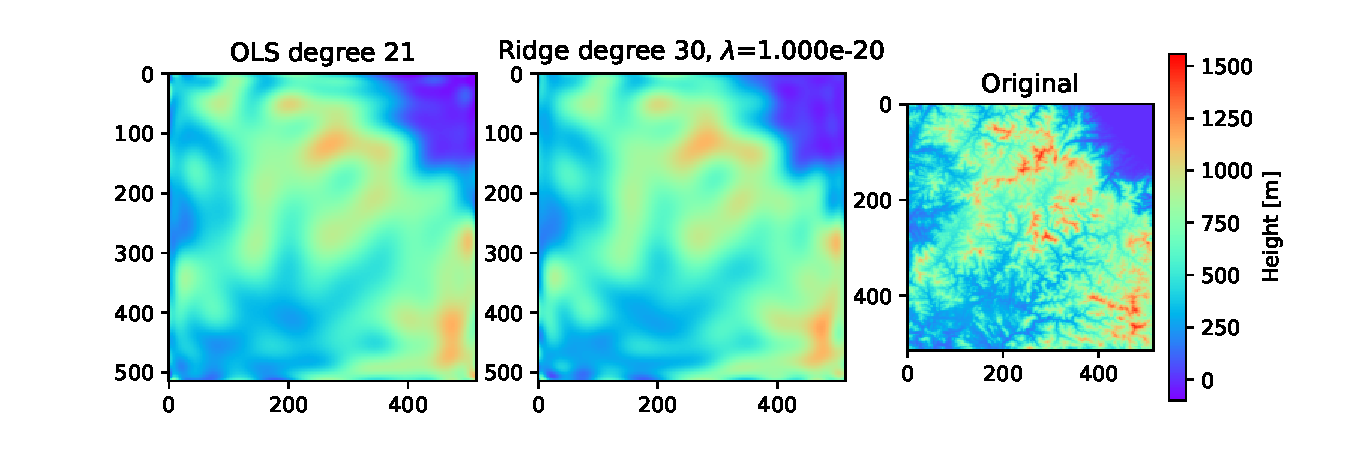
\includegraphics[width=1.0\textwidth]{Fitted_images.pdf}
\caption[Fitted geodata with 20000 points]{Fit of the geodata with parameters that reduce the MSE using Ridge regression and OLS regression. The original (scaled) image is included as well. 20,000 data points were used.}
\label{fig:Korea_plot}
\end{figure}
\begin{figure}[H]
\centering
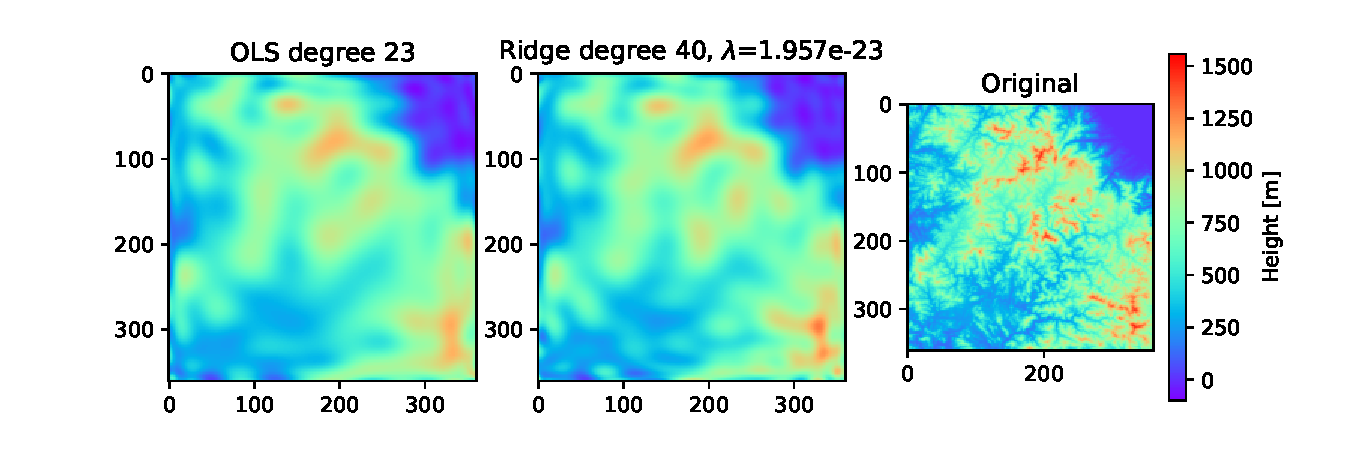
\includegraphics[width=1.0\textwidth]{Fitted_imagesKorea50000_NOBOOTSTRAP.pdf}
\caption[Fitted geodata with 50000 points]{Fit of the geodata with parameters that reduce the MSE using Ridge regression and OLS regression. The original (scaled) image is included as well. 50,000 data points were used.}
\label{fig:Korea_plot_XXL}
\end{figure}
Just from these pictures, we can see a lot. Both the OLS and the Ridge fit manage to fit the area in such a way that is generally correct - the large mountain ranges and the deep valleys are included, the sea is the "deepest" part, and of course, the dimensions are correct. We also see how having a larger sample set increases the quality of the fit - there are more details in figure \ref{fig:Korea_plot_XXL} that lack in figure \ref{fig:Korea_plot}.  However, there is a profound lack of detail both in the OLS and in the Ridge fit. Even the "easy" part (the dark area, which symbolizes the sea) is not very well fitted (it goes below zero), which lies in the nature of a polynomial fit. This is rather frustrating, as both creating these images and finding the ideal parameters is very time-consuming. Increasing the data points would give an even better result, but by the fact that the MSE is above 15,000, it is unlikely that there is a huge improvement. A MSE of 15,000 means that the minimal root MSE is around 120, which, while different from the Mean Absolute Error, still gives an indication on the "average difference" between the original data and our fit. All of this combined shows that Regression is not the ideal way to match such complex data where there does not seem to exist a functional relationship with little error. 
\section{Conclusion}
Our analysis of methods has given a lot of insight. First of all, fitting a "simple" function such as the  Franke function, can be done with little loss using any of the methods, especially when the underlying error is small. Sadly, this cannot be said about complex data such as the geographic data, where it was not possible to predict more than the most basic traits due to the nature of the data, making it look like a picture from the late 18th century. OLS seems to be sufficient for fitting the Franke Function, but Ridge Regression performed much better on the geographic data. However, OLS is computationally cheaper, but on the other hand, OLS is prone to overfitting, which is not the case with Ridge regression. LASSO is a very expensive method due to the lack of an analytical solution, and in this analysis, it has been prohibitively expensive. Finding the parameter $\lambda$ by iterating over all values is very expensive, and using more clever methods is necessary in large-scale projects. \\
Error estimation is no easy task, and two of the most used methods give different error estimates - while they are in the same magnitude, they do differ largely, especially where there are steep changes. k-fold Cross Validation is the preferred method for large projects, especially when using numerical solvers such as we did for LASSO regression - this is because the Bootstrap method can be extremely slow.
\section{Appendix}
\subsection{Proof that the MSE can be decomposed into Bias and Variance}
\begin{equation}\label{Proof}
\begin{split}
MSE(y,\tilde y) & =\mathbb{E}\left[({y}-{\tilde y})^2  \right] \\
&= \mathbb{E}\left[({f}+{\epsilon}-\mathbb{E}\left[\tilde y\right]+\mathbb{E}\left[\tilde y\right]-{\tilde y})^2  \right]\\
&= \mathbb{E}\left[(f+\epsilon- \mathbb{E}\left[\tilde y\right])^2+(\mathbb{E}\left[\tilde y\right]-{\tilde y})^2 \right]+2\mathbb{E}\left[(f+\epsilon-\mathbb{E}\left[\tilde y\right])(\mathbb{E}\left[\tilde y\right]-\tilde y)\right]\\
&= \mathbb{E}\left[\epsilon^2\right]+\mathbb{E}\left[(f-\mathbb{E}\left[\tilde y\right])^2\right]+\mathbb{E}\left[ \mathbb{E}\left[\tilde y\right]-\tilde y)^2\right]\\   & +2\mathbb{E}\left[\epsilon\right]\mathbb{E}\left[f-\mathbb{E}\left[\tilde y\right]\right]+2\mathbb{E}\left[(f-\mathbb{E}\left[\tilde y\right])(\mathbb{E}\left[\tilde y\right]-\tilde y)\right] +2\mathbb{E}\left[\epsilon (\mathbb{E}\left[\tilde y\right]-\tilde y)\right] \\ 
&=\sigma^2+Bias(\tilde y)^2+Var(\tilde y) \\ &
+2\mathbb{E}\left[\epsilon\right]\mathbb{E}\left[f-\mathbb{E}\left[\tilde y\right]\right]+2\mathbb{E}\left[(f-\mathbb{E}\left[\tilde y\right])(\mathbb{E}\left[\tilde y\right]-\tilde y)\right] +2\mathbb{E}\left[\epsilon (\mathbb{E}\left[\tilde y\right]-\tilde y)\right] \\
&=\sigma^2+Bias(\tilde y)^2+Var(\tilde y) \\ &
+2\mathbb{E}\left[\epsilon\right]\mathbb{E}\left[f-\mathbb{E}\left[\tilde y\right]\right]+2(f-\mathbb{E}\left[\tilde y\right])\mathbb{E}\left[(\mathbb{E}\left[\tilde y\right]-\tilde y)\right] +2\mathbb{E}\left[\epsilon\right]\mathbb{E}\left[ (\mathbb{E}\left[\tilde y\right]-\tilde y)\right]\\
&=\sigma^2+Bias(\tilde y)^2+Var(\tilde y)
\end{split}
\end{equation}
where we used that $\mathbb{E}\left[\epsilon\right]=0$, that $(f-\mathbb{E}\left[\tilde y\right])$ simply is a number (as f is deterministic) and that $\epsilon$ and $\tilde y$ are independent variables (hence the expected value can be separated), as well as the fact that $\mathbb{E}\left[\mathbb{E}\left[\tilde y\right]-\tilde y\right]=\mathbb{E}\left[\tilde y\right]-\mathbb{E}\left[\tilde y\right]=0$ 
\subsection{Figures}
\begin{figure}[H]
\centering
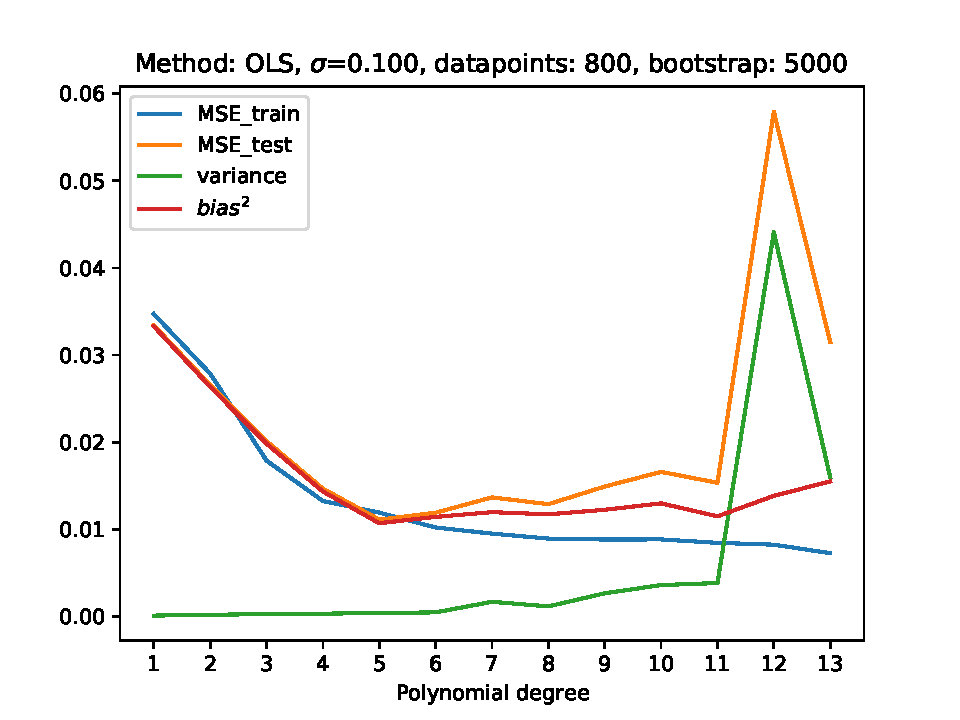
\includegraphics[width=0.65\textwidth]{Bias_Variance_OLS_BAD.pdf}
\caption[Bias, Variance, MSE \& training MSE as a function of the polynomial degree using OLS regression - whacky version]{Bias, Variance, MSE \& training MSE as a function of the polynomial degree using OLS regression. The values for $\sigma$, the size of the dataset and the number of bootstraps can be found in the title. As one can see, the chosen parameters lead to a rather "jumpy" bias and an increasing, then decreasing, variance and an increasing variance.}
\label{fig:Bias_Variance_fucked}
\end{figure}
\bibliographystyle{plain}
\bibliography{references}
\end{document}
$2\mathbb{E}\left[\epsilon\right]$
